\documentclass[bachelor, och, coursework]{SCWorks}
% параметр - тип обучения - одно из значений:
%    spec     - специальность
%    bachelor - бакалавриат (по умолчанию)
%    master   - магистратура
% параметр - форма обучения - одно из значений:
%    och   - очное (по умолчанию)
%    zaoch - заочное
% параметр - тип работы - одно из значений:
%    referat    - реферат
%    coursework - курсовая работа (по умолчанию)
%    diploma    - дипломная работа
%    pract      - отчет по практике
% параметр - включение шрифта
%    times    - включение шрифта Times New Roman (если установлен)
%               по умолчанию выключен
\usepackage{subfigure}
\usepackage{tikz,pgfplots}
\pgfplotsset{compat=1.5}
\usepackage{float}

%\usepackage{titlesec}
\setcounter{secnumdepth}{4}
%\titleformat{\paragraph}
%{\normalfont\normalsize}{\theparagraph}{1em}{}
%\titlespacing*{\paragraph}
%{35.5pt}{3.25ex plus 1ex minus .2ex}{1.5ex plus .2ex}

\titleformat{\paragraph}[block]
{\hspace{1.25cm}\normalfont}
{\theparagraph}{1ex}{}
\titlespacing{\paragraph}
{0cm}{2ex plus 1ex minus .2ex}{.4ex plus.2ex}

% --------------------------------------------------------------------------%


\usepackage[T2A]{fontenc}
\usepackage[utf8]{inputenc}
\usepackage{graphicx}
\graphicspath{ {./images/} }
\usepackage{tempora}

\usepackage[sort,compress]{cite}
\usepackage{amsmath}
\usepackage{amssymb}
\usepackage{amsthm}
\usepackage{fancyvrb}
\usepackage{listings}
\usepackage{listingsutf8}
\usepackage{longtable}
\usepackage{array}
\usepackage[english,russian]{babel}

% \usepackage[colorlinks=true]{hyperref}
\usepackage{url}

\usepackage{underscore}
\usepackage{setspace}
\usepackage{indentfirst} 
\usepackage{mathtools}
\usepackage{amsfonts}
\usepackage{enumitem}
\usepackage{tikz}
\usepackage{minted}

\newcommand{\eqdef}{\stackrel {\rm def}{=}}
\newcommand{\specialcell}[2][c]{%
\begin{tabular}[#1]{@{}c@{}}#2\end{tabular}}

\renewcommand\theFancyVerbLine{\small\arabic{FancyVerbLine}}

\newtheorem{lem}{Лемма}

\begin{document}

% Кафедра (в родительном падеже)
\chair{теоретических основ компьютерной безопасности и криптографии}

% Тема работы
\title{Статистический анализ сетевого трафика для обнаружения активной RDP-сессии}

% Курс
\course{4}

% Группа
\group{431}

% Факультет (в родительном падеже) (по умолчанию "факультета КНиИТ")
\department{факультета КНиИТ}

% Специальность/направление код - наименование
%\napravlenie{09.03.04 "--- Программная инженерия}
%\napravlenie{010500 "--- Математическое обеспечение и администрирование информационных систем}
%\napravlenie{230100 "--- Информатика и вычислительная техника}
%\napravlenie{231000 "--- Программная инженерия}
\napravlenie{10.05.01 "--- Компьютерная безопасность}

% Для студентки. Для работы студента следующая команда не нужна.
% \studenttitle{Студентки}

% Фамилия, имя, отчество в родительном падеже
\author{Токарева Никиты Сергеевича}

% Заведующий кафедрой
\chtitle{} % степень, звание
\chname{Абросимов М. Б.}

%Научный руководитель (для реферата преподаватель проверяющий работу)
\satitle{доцент} %должность, степень, звание
\saname{Гортинский А. В.}

% Руководитель практики от организации (только для практики,
% для остальных типов работ не используется)
% \patitle{к.ф.-м.н.}
% \paname{С.~В.~Миронов}

% Семестр (только для практики, для остальных
% типов работ не используется)
%\term{8}

% Наименование практики (только для практики, для остальных
% типов работ не используется)
%\practtype{преддипломная}

% Продолжительность практики (количество недель) (только для практики,
% для остальных типов работ не используется)
%\duration{4}

% Даты начала и окончания практики (только для практики, для остальных
% типов работ не используется)
%\practStart{30.04.2019}
%\practFinish{27.05.2019}

% Год выполнения отчета
\date{2023}

\maketitle

% Включение нумерации рисунков, формул и таблиц по разделам
% (по умолчанию - нумерация сквозная)
% (допускается оба вида нумерации)
% \secNumbering

%-------------------------------------------------------------------------------------------

\tableofcontents

\intro
Сегодня удаленный доступ к компьютерам является важным элементом современного мира. Сотрудники компаний могут работать на расстоянии, а 
IT-специалисты могут удаленно управлять компьютерами, находящимися в другой стране. Однако, в то же время, удаленный доступ может стать 
уязвимостью компьютерной системы. Один из наиболее распространенных протоколов для удаленного доступа является RDP (Remote Desktop Protocol). 

Цель данной курсовой работы --- разработка метода статистического анализа сетевого трафика для обнаружения активной RDP-сессии. 
Будут использованы статистические методы анализа, такие как распределение временных интервалов между пакетами, нахождение стандартного отклонения и 
среднего значения, для выявления характеристик, свойственных протоколу RDP.

В работе будет представлено описание алгоритма, позволяющего производить статистический анализ сетевого трафика для обнаружения активной 
RDP-сессии, а также оценка эффективности методов на реальных сетевых данных. 
Результаты данной работы могут быть использованы в качестве инструмента для мониторинга сетевого трафика.


\section{Определение RDP}

  Протокол RDP (от англ. Remote Desktop Protocol --- протокол удалённого рабочего стола) --- патентованный протокол 
  прикладного уровня компании Microsoft и приобретен ею у другой компании Polycom, который предоставляет пользователю графический интерфейс для 
  подключения к другому компьютеру через сетевое соединение. Для этого пользователь запускает клиентское программное обеспечение RDP, а на другом 
  компьютере должно быть запущено программное обеспечение сервера RDP \cite{2}.

  Стоит отметить, что RDP позволяет работать с удаленным компьютером, почти как с локальным. При успешном создании RDP-сессии пользователь может
  двигать мышкой, открывать файлы, диски, документы, программы, без каких-либо проблем использовать буфер обмена (Ctrl+C, Ctrl+V) не только для текста, 
  но и для файлов. Также отлично работает передача сочетаний клавиш, переключения языков.

  \subsection{Место протокола RDP в структуре OSI}

    Эталонная модель OSI представляет собой 7-уровневую иерархическую сетевую иерархию, разработанную международной организацией по стандартам
    (International Standardization Organization --- ISO). В рамках модели, любой протокол может взаимодействовать либо с протоколами своего
    уровня (горизонтальные взаимодействия), либо с протоколами уровня на единицу выше/ни-\\*же своего уровня (вертикальные взаимодействия).
    Каждый из семи уровней характеризуется типом данных, которым данный уровень оперирует и функционалом, который он предоставляет слою,
    находящемуся выше него \cite{osi-model}. Модель OSI включает в себя следующие уровни:

    \begin{enumerate}
      \item Физический уровень, который отвечает за передачу последовательности битов через канал связи;
      \item Канальный уровень, где осуществляется разбиение данных на <<кадры>>, размер которых обычно достигает
      от несколько сотен до нескольких тысяч байтов;
      \item Сетевой уровень, на котором осуществляется структуризация и маршрутизация пакетов от отправителя к получателю;
      \item Транспортный уровень, функцией которого является передача надежных последовательностей данных произвольной
      длины через коммуникационную сеть от отправителя к получателю;
      \item Сеансовый уровень, на котором происходит поддержка сессии связи, уп-\\*равление взаимодействием между приложениями;  
      \item Уровень представления, который представляет данные в понятном для какой-либо конкретной машины виде;
      \item Прикладной уровень, предоставляющий набор интерфейсов для взаимодействия пользовательских процессов с сетью.
    \end{enumerate}

    Вследствие этого, RDP является непосредственно протоколом прикладного уровня модели OSI, наряду с SMTP, HTTP, FTP и многими другими. 
    Протоколы седьмого уровня используют TCP или UDP в качестве передачи информации. Поэтому данные протокола RDP хранятся в заголовках TCP и
    UDP. 
    
    Далее для понимания того, в каком виде информация передается от отправителя к получателю необходимо разобрать структуру пакета.
    Согласно вышесказанному с помощью протоколов TCP и UDP отправитель передает данные, принадлежащие RDP, получателю. Они хранятся в специальном поле данных.
    Его можно увидеть на рисунке \ref{tcp-header}, где изображена структура TCP-заголовка.
    
      \begin{figure}[H]
        \centering
        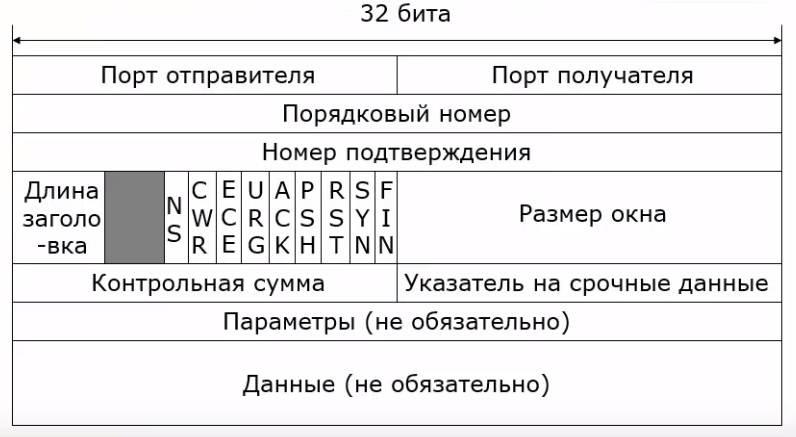
\includegraphics[width=0.9\textwidth]{photo/tcp-segment.jpg}
        \caption{Структура TCP-заголовка}
        \label{tcp-header}
      \end{figure}
      
    Помимо поля данных в TCP-заголовке для дальнейшего анализа будут интересными поля, в которых хранится информация о портах отправителя и получателя.
    Стоит отметить, что при подключении к удаленному рабочему столу по умолчанию используется порт 3389. Поэтому для обнаружения RDP-сессии
    информация о портах будет достаточно полезной.

    Также не менее интересной информацией являются установленные флаги, хранящиеся в поле флагов. В нем хранятся следующие управляющие биты:

    \begin{enumerate}
      \item NS --- одноразовая сумма (Nonce Sum). По-прежнему является экспериментальным флагом, используемым для защиты от случайного
      злонамеренного сокрытия пакетов от отправителя \cite{tcpflags}. Используется для улучшения работы механизма явного уведомления 
      о перегрузке (Explicit Congestion Notification, ECN);
      \item CWR --- окно перегрузки уменьшено (Congestion Window Reduced). 
      Данный флаг устанавливается (принимает значение равной единице) отправителем, чтобы показать, что TCP-фрагмент был
      получен с установленным полем ECE;
      \item ECE --- ECN-Эхо (ECN-Echo). Этот флаг показывает, поддерживает ли TCP-отправитель ECN;
      \item URG --- устанавливается, если необходимо передать ссылку на поле указателя срочности (Urgent pointer);
      \item ACK --- флаг подтверждения используется для подтверждения успешного получения пакета;
      \item PSH --- инструктирует получателя протолкнуть данные, накопившиеся в приемном буфере, в приложение пользователя;
      \item RST --- флаг сброса отправляется от получателя к отправителю, когда пакет отправляется на конкретный хост, который этого не ожидал;
      \item SYN --- начинает соединение и синхронизирует порядковые номера. Первый пакет, отправленный с каждой стороны, должен в обязательном порядке иметь установленным этот флаг;
      \item FIN --- означает, что данных от отправителя больше нет. Поэтому он используется в последнем пакете, отправленном отправителем.
    \end{enumerate}


    Благодаря вышеописанным флагам можно узнать информацию о конкретном состоянии соединения.
    
    IP пакет представляет собой отформатированную информацию в блоке, которая передается в сети. В настоящее время применяются две версии IP пакетов: IPv4 и IPv6.    
    В данной работе будут рассматриваться пакеты IP версии 4, 
    так как для анализа данных этого вполне достаточно. Поэтому далее необходимо рассмотреть IPv4-заголовок, который показан на рисунке \ref{ipv4-header}.

    \begin{figure}[H]
      \centering
      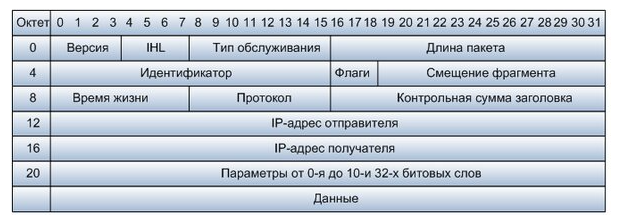
\includegraphics[width=0.9\textwidth]{photo/ipv4-header.png}
      \caption{Структура IPv4-заголовка}
      \label{ipv4-header}
    \end{figure}

    IPv4 используется на сетевом уровне модели OSI для осуществления передачи пакетов между сетями.

    В его заголовке достаточно важной информацией являются поля, в которых записаны IP-адреса отправителя и получателя. Ведь благодаря этой информации можно
    определить, между какими устройствами происходит обмен данными.

    Также необходимо обратить внимание на 8-разрядное поле протокола. На рисунке оно обозначено как <<Протокол>>. С помощью него можно 
    идентифицировать протоколы следующего уровня (TCP, UDP, ICMP и другие) по его номеру. Например, если в IPv4-заголовке в поле <<Протокол>> 
    будет задан номер 6, значит в поле данных хранится информация о протоколе TCP.
    
    Согласно модели OSI, если перейти на один уровень ниже, а именно на канальный, то на нем осуществляется инкапсуляция пакета, полученного на сетевом уровне, где
    добавляется дополнительный заголовок, кадр Ethernet, к сегменту данных. Его структура показана на рисунке \ref{eth-frame}.

    \begin{figure}[H]
      \centering
      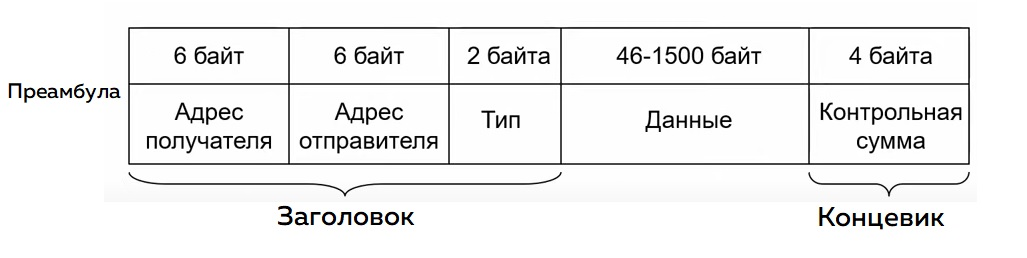
\includegraphics[width=0.9\textwidth]{photo/eth-frame.jpg}
      \caption{Структура Ethernet кадра}
      \label{eth-frame}
    \end{figure}

    Здесь достаточно важной информацией считаются поля адресов отправителя и получателя.
    Ведь в них содержатся MAC-адреса источника и назначения соответственно.
    В поле <<Тип>>, содержится номер, идентифицирующий тип сетевого протокола. 
    Также в поле данных содержатся данные от более высокого уровня согласно модели OSI, а именно инкапсулированные данные о пакете.

    Далее необходимо рассмотреть методы обнаружения RDP-трафика, которые позволят эффективно выявить наличие использования RDP-протокола.


\section{Обзор существующих методов обнаружения RDP-трафика}

%RDP (Remote Desktop Protocol) --- это протокол удаленного рабочего стола, который используется для удаленного управления компьютерами. 
%Протокол RDP позволяет пользователям подключаться к удаленному компьютеру, используя протокол TCP/IP и передавать данные через сеть.

Обзор существующих методов обнаружения RDP-трафика представляет собой анализ различных подходов и техник, применяемых для выявления 
использования RDP-протокола в сетевом трафике.

Существует несколько методов обнаружения RDP-трафика, которые могут использоваться для мониторинга сети и выявления потенциальных угроз:

\begin{enumerate}
  \item Анализ портов: RDP-протокол обычно использует TCP-порт 3389, поэтому можно использовать анализ портов для обнаружения трафика, 
  проходящего через этот порт.
  \item Поиск заголовков пакетов: RDP-протокол имеет уникальную сигнатуру в заголовке пакетов, которые могут быть использованы для 
  обнаружения его наличия в сети.
  \item Машинное обучение: Машинное обучение может быть использовано для создания моделей, которые могут обнаруживать RDP-трафик на 
  основе статистических данных и образцов поведения сети.
  \item Анализ временных интервалов: Временные интервалы между пакетами RDP-трафика обычно меньше, чем между другими типами трафика, 
  что можно использовать для обнаружения RDP-сессий.
  \item Анализ размеров пакетов: Размеры пакетов RDP-трафика обычно больше, чем у других типов трафика, что также может помочь в 
  обнаружении RDP-сессий.
  \item Анализ флагов пакетов: определенные флаги пакетов могут указывать на использование RDP-протокола. Например, флаг PSH может 
  указывать на передачу данных в реальном времени в рамках RDP-сессии.
\end{enumerate}

Хотя все вышеперечисленные методы обнаружения RDP-трафика могут быть полезными инструментами для обнаружения RDP-сессии, но ни один из них 
не является идеальным.

Если брать в рассмотрение анализ портов, то этот метод неэффективен по нескольким причинам. Во-первых, злоумышленники могут изменить порт, 
используемый для RDP-соединения, чтобы избежать обнаружения. Во-вторых, если на одном компьютере работает несколько RDP-сессий, они могут 
использовать разные порты, что затрудняет обнаружение RDP-трафика на основе порта. В-третьих, RDP-трафик может быть запакован в другой 
протокол, который использует другой порт, что также затрудняет обнаружение по порту.

Поиск заголовков пакетов также может быть ненадежным методом обнаружения RDP-трафика, потому что некоторые приложения могут использовать 
измененные заголовки, чтобы скрыть свой трафик. Кроме того, если RDP-трафик зашифрован, то заголовки пакетов могут быть недоступны для 
анализа. Также возможно наличие поддельных заголовков, созданных злоумышленниками для обхода системы обнаружения RDP-трафика. Все это 
делает поиск заголовков пакетов не надежным методом для обнаружения RDP-трафика в некоторых случаях.

При использовании машинного обучения для обнаружения RDP-трафика может возникнуть ряд проблем:

\begin{enumerate}
  \item Необходимость большого объема данных: Для того чтобы создать надежную модель машинного обучения для обнаружения RDP-трафика, 
  требуется большой объем данных для обучения. Данные должны включать в себя как положительные, так и отрицательные примеры RDP-трафика, 
  что может быть сложно собрать.
  \item Низкая точность: Машинное обучение может иметь низкую точность при обнаружении RDP-трафика из-за возможных ошибок классификации. 
  Например, некоторые другие протоколы могут иметь схожие характеристики с RDP-трафиком, что может привести к неверной классификации.
  \item Низкая скорость: Машинное обучение может быть времязатратным процессом. Обучение модели может занять много времени и требовать 
  больших вычислительных ресурсов.
  \item Адаптация к новым типам RDP-трафика: Машинное обучение может не справиться с обнаружением новых типов RDP-трафика, которые 
  отличаются от тех, которые были использованы при обучении модели.
\end{enumerate}

Все эти факторы могут привести к тому, что машинное обучение не будет надежным методом обнаружения RDP-трафика. Однако, если используется 
достаточно объемный и репрезентативный набор данных для обучения, а также проводится тщательное тестирование модели, то машинное обучение
может быть эффективным методом обнаружения RDP-трафика.



Стоит отметить, что каждый из методов анализа временных интервалов, размеров пакетов и флагов пакетов имеет свои собственные недостатки. 
Тем не менее, все три метода могут быть реализованы совместно. 

Основная часть работы состояла из двух этапов. На первом этапе был разработан сниффер, предназначенный для перехвата сетевого трафика. 
В рамках этого этапа были созданы функции записи и чтения сетевого трафика в файл, а также возможность построения графиков, которые 
позволяли просмотреть сетевой трафик относительно заданного IP-адреса и порта, и проведения статистической обработки этих параметров.

На втором этапе были применены эффективные преобразования признаков, которые внедрены в программу как средства оценки вероятности наличия 
протокола RDP. Кроме того, проводилась калибровка граничных значений. 

Далее в курсовой работе будет представлен обзор программы <<traffic-detection.py>>, в котором будут описаны ее основные возможности. 
Затем будет подробно рассмотрен каждый из статистических методов анализа сетевого трафика, которые были внедрены в данную программу. 
В конце работы будут представлены результаты нескольких тестов, проведенных с использованием программы <<traffic-detection.py>>.


\section{Программная реализация метода обнаружения RDP-трафика}

При запуске программы <<traffic-detection.py>> пользователю предоставляется выбрать одну из следующих опций:

\begin{enumerate}
  \item Перехват трафика: при выборе данной опции происходит перехват трафика с помощью сниффера, программного обеспечения, которое анализирует входящий
  и исходящий трафик с компьютера. Далее пользователю предлагают установить RDP-фильтр при осуществлении перехвата трафика, как показано на рисунке 
  \ref{cmd-filter}.
  
  \begin{figure}[H]
    \centering
    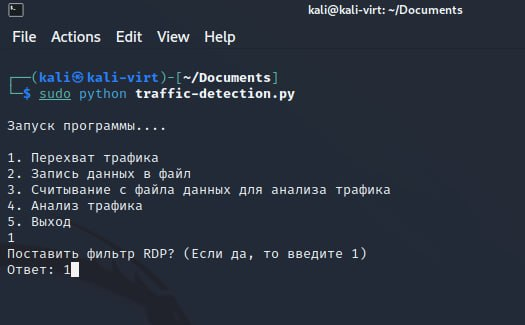
\includegraphics[width=0.6\textwidth]{photo/cmd-filter.jpg}
    \caption{Вид консоли при выборе опции <<Перехват трафика>>}
    \label{cmd-filter}
  \end{figure}

  Если ввести в консоль цифру <<1>>, то программа будет выводить информацию только о тех перехваченных пакетах, которые содержат признаки протокола RDP. 
  Если пользователь не вводит никаких цифр и оставляет поле ввода пустым, то в консоли будут отображаться все пакеты, которые перехватывает сниффер.
  Также пользователю нужно выбрать сетевой интерфейс, по которому производится перехват трафика, как показано на следующем рисунке.


  \begin{figure}[H]
    \centering
    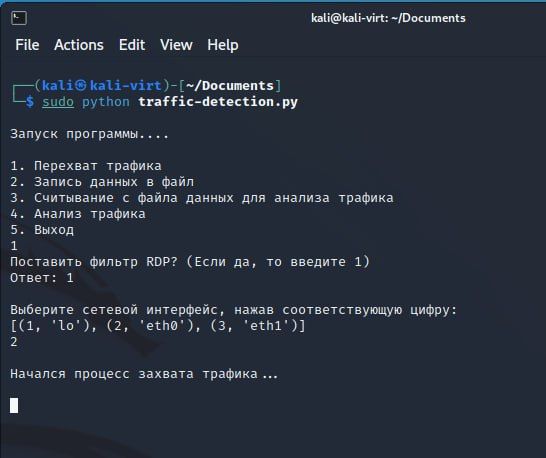
\includegraphics[width=0.6\textwidth]{photo/cmd-start.jpg}
    \caption{Выбор интерфейса и начало перехвата трафика}
    \label{cmd-start}
  \end{figure}


  Чтобы остановить перехват сетевого трафика, необходимо нажать клавишу <<пробел>>. После завершения перехвата трафика пользователю предлагают ввести
  название файла, чтобы записать информацию о всех перехваченных пакетов в файл, как показано на рисунке \ref{sniff-fin}.


  \begin{figure}[H]
    \centering
    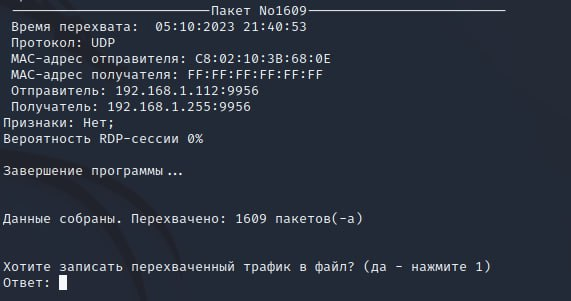
\includegraphics[width=0.6\textwidth]{photo/sniff-fin.jpg}
    \caption{Завершение перехвата трафика после нажатия клавиши <<пробел>>}
    \label{sniff-fin}
  \end{figure}


  \item Запись данных в файл: если в результате перехвата трафика было захвачено несколько пакетов, то можно записать всю перехваченную информацию в 
  файл, введя имя файла. Добавление этой опции было целью расширения возможностей пользователя по сохранению данных в файл. 
  \item Считывание с файла для анализа данных: для анализа данных можно использовать опцию считывания информации из файла. 
  Она позволяет извлекать только ту информацию о пакетах, которая была предварительно записана с помощью программы <<traffic-detection.py>>.
  \item Анализ трафика: когда пользователь выбирает данную опцию, программа выводит в консоль информацию о всех возможных сессиях, которые продлились 
  более 10 секунд в момент перехвата трафика. Обнаружение этих сессий будет описано позже. Выводится также некоторая общая информация о перехваченном 
  трафике, такая как время начала и завершения перехвата трафика, количество пакетов, среднее количество пакетов в секунду и средний размер пакетов. 
  Кроме того, выводится список IP-адресов, участвующих в передаче пакетов по сети, как показано на рисунке \ref{cmd-geninf}. 
  
  \begin{figure}[H]
    \centering
    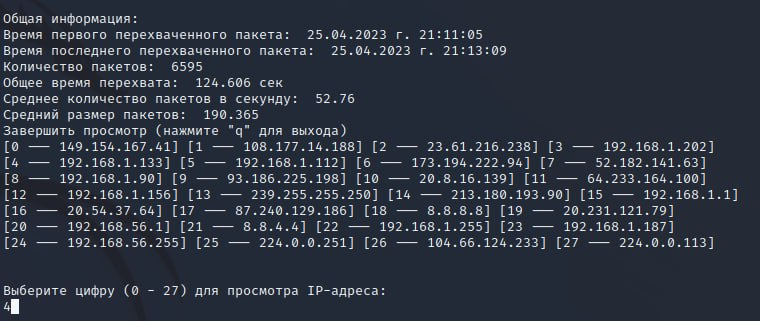
\includegraphics[width=0.7\textwidth]{photo/cmd-geninf.jpg}
    \caption{Вывод общей информации о перехваченном трафике}
    \label{cmd-geninf}
  \end{figure}


  Пользователь может выбрать интересующий его IP-адрес для дальнейшего анализа пакетов, связанных с ним. После выбора 
  IP-адреса пользователю предоставляется выбор конкретного порта, по которому выбранный IP-адрес осуществлял передачу сообщений, 
  как показано на рисунке \ref{cmd-geninf1}.
  
  \begin{figure}[H]
    \centering
    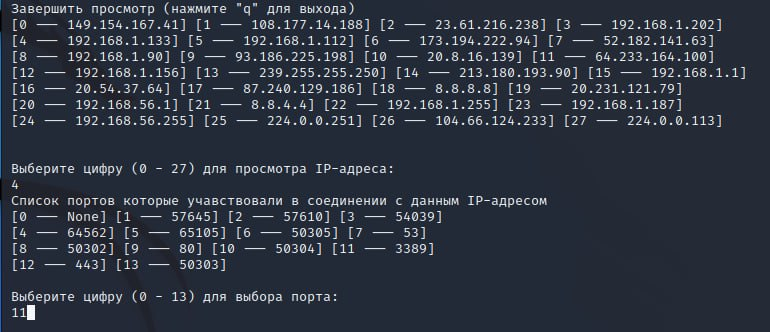
\includegraphics[width=0.7\textwidth]{photo/cmd-geninf1.jpg}
    \caption{Вывод информации о портах относительно конкретного IP-адреса}
    \label{cmd-geninf1}
  \end{figure}

  Затем выводится общая информация только относительно выбранного IP-адреса и порта, такая 
  как время первого и последнего перехваченных пакетов, где данный IP-адрес выступает в качестве отправителя или получателя.
  Таким образом можно понять, в какой конкретно момент времени начался обмен информацией с тем или иным IP-адресом.

  После вывода общей информации пользователю предоставляется следующий функционал:

  \begin{enumerate}
    \item Вывод сетевого трафика, где в качестве отправителя или получателя выступает выбранный IP-адрес.
    \item Построение графика отношения объема входящего трафика и исходящего трафика в единицу времени. Данное отношение 
    рассчитывается по формуле
    
    \begin{center}
      $r_{ip} = \frac{V_{dest}}{V_{src}}$,
    \end{center}

    где $V_{dest}$ и $V_{src}$ --- объемы соответственно входящего и исходящего трафика в единицу времени. 


    \item Построение графика отношения $V_{udp}$ --- объема входящего UDP-трафика и $V_{tcp}$ объема входящего TCP-трафика.
    Отношение рассчитывается по формуле

    \begin{center}
      $r_{udp} = \frac{V_{udp}}{V_{tcp}}$.
    \end{center}

    Стоит отметить, что во время RDP-сессии передача пакетов может осуществляться по протоколам UDP и TCP. Хотя в большинстве программ удаленного
    рабочего стола передача сообщений происходит только по протоколу TCP. Однако существуют до сих пор приложения, которые используют и протокол
    UDP, и пртокол TCP. Например, приложение ОС Windows <<Подключение к удаленному рабочему столу>> (Remote Desktop Connection, RDC) использует для
    передачи пакетов по-умолчанию оба транспортных протокола. Это сделано для того чтобы оптимизировать передачу данных, обеспечивая надежную 
    доставку управляющих сообщений и минимизируя задержки при передаче потоковых данных.
    
    \item Построение графика разности количества исходящих и входящих TCP-пакетов, в которых флаг ACK имеет значение
    равное единице.

    \begin{center}
      $r_{ack} = V_{A_{out}} - V_{A_{in}}$,
    \end{center}

    где $V_{A_{in}}$ и $V_{A_{out}}$ --- число входящих и исходящих ACK-флагов в TCP-трафике в единицу времени. При подключении к удаленному рабочему 
    столу сервер отправляет клиенту TCP-пакеты с установленным флагом ACK, указывающим, что поле номера подтверждения задействовано. Изменяясь во времени, 
    значение $r_{ack}$ может использоваться для определения активной сессии в определенные моменты времени с помощью графика.

    \item Построение двух графиков, показывающих частоту SYN-флагов и PSH-флагов в TCP-трафике. Частота SYN-флагов находится по формуле
    
    \begin{center}
      $r_{syn} = \frac{V_{S_{in}}}{V_{tcp}}$,
    \end{center}

    где $V_{S_{in}}$ число входящих TCP-пакетов, в которых установлен флаг SYN = 1, $V_{tcp}$ --- число входящих TCP-пакетов в единицу времени.
    В процессе установления TCP-соединения между клиентом и сервером передаются пакеты с флагом SYN, а обмен данными начинается с 
    использованием пакетов без этого флага. Таким образом, количество SYN-флагов, полученных сервером, соответствует числу запросов 
    на соединение, а частота их появления определяет долю служебных пакетов этого типа в TCP-трафике.

    Частота PSH-флагов вычисляется по формуле 
    
    \begin{center}
      $r_{psh} = \frac{V_{P_{in}}}{V_{tcp}}$,
    \end{center}
    
    где $V_{P_{in}}$ число входящих TCP-пакетов, в которых установлен флаг PSH = 1, $V_{tcp}$ --- число входящих TCP-пакетов в единицу времени.
    Флаг PSH (Push) в TCP-заголовке используется для указания конечной точке передачи данных о том, что все буферизованные данные должны быть 
    немедленно отправлены получателю, а не ждать буферизации следующих данных. Когда отправитель устанавливает флаг PSH в заголовке TCP-сегмента, 
    он указывает получателю, что данные в этом сегменте должны быть переданы верхнему уровню протокола немедленно, без буферизации на приемной стороне.
    Таким образом, если значение величины $r_{psh}$ резко возросло в некоторый промежуток времени, значит за это время
    одно устройcтво успело передать другому устройству большое количество пакетов.

    \item Для получения представления о количестве передачи пакетов в сети были построены два графика: один показывает количество входящих пакетов 
    в единицу времени, а другой --- исходящих. Таким образом, эти графики позволяют оценить количество передаваемых пакетов в сети в единицу времени.
    \item Построение двух графиков, показывающих максимальные размеры входящих и исходящих пакетов в единицу времени. Эти графики показывают, какие 
    максимальные размеры пакетов передаются по сети в каждую секунду.
    \item Последняя опция позволяет пользователю вернуться к выбору другого IP-адреса.

    Перед построением каждого графика пользователю предоставляется возможность добавить второй IP-адрес, с которым выбранный IP-адрес взаимодействовал 
    в момент перехвата трафика, как показано на рисунке \ref{cmd-2ndip}.

    \begin{figure}[H]
      \centering
      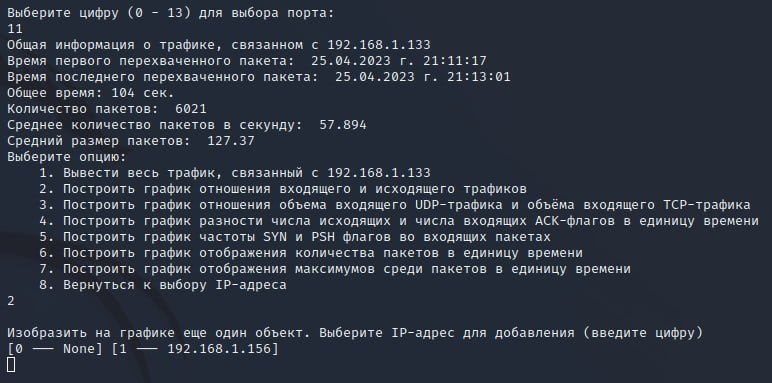
\includegraphics[width=0.7\textwidth]{photo/cmd-2ndip.jpg}
      \caption{Предоставление пользователю возможности выбрать второй IP-адрес}
      \label{cmd-2ndip}
    \end{figure}

    Если пользователь выбирает второй IP-адрес, появляется новое окно, в котором отображаются данные о двух графиках.
    В противном случае появляется окно, где изображены данные только об одном ранее выбранном IP-адресе. 

  \end{enumerate}


  \item Выход: при выборе данной опции программа <<traffic-detection.py>> завершает свою работу.
\end{enumerate}

% \subsection{Инструменты для захвата сетевого трафика}
\subsection{Определение активных сессий путем анализа TCP-соединения}

Как уже упоминалось ранее при выборе опции <<Анализ трафика>> появляется информация об активных сессиях, как показано на следующем рисунке.

\begin{figure}[H]
  \centering
  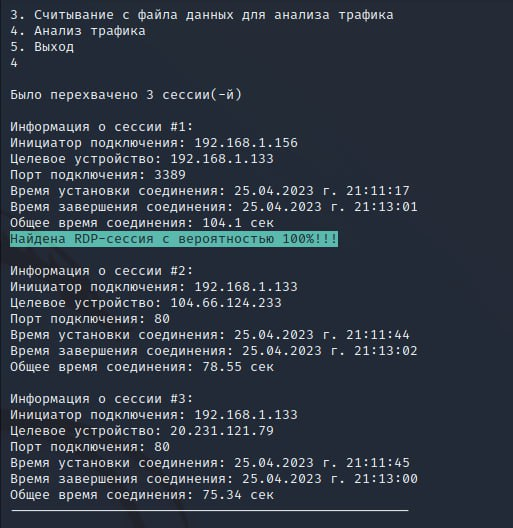
\includegraphics[width=0.7\textwidth]{photo/cmd-activeses.jpg}
  \caption{Вывод информации об активных сессиях}
  \label{cmd-activeses}
\end{figure}

Под активной сесией будем понимать связь между двумя устройствами, в которой происходит обмен данными. В сетевом трафике, активная сессия 
обычно определяется как установленное соединение между двумя устройствами, которое использует определенный протокол для передачи данных.
Активная сессия образуется при установке TCP-соединения. Такой процесс также называют <<трехсторонним рукопожатием>> (Three-way Handshake). Он состоит 
из следующих этапов:

\begin{enumerate}
  \item Клиент отправляет серверу пакет с установленным флагом SYN (Synchronize Sequence Number), который указывает на начало соединения. В этом 
  пакете клиент выбирает начальное значение порядкового номера (sequence number), которое будет использоваться в дальнейшем.
  \item Сервер получает пакет с флагом SYN и отвечает на него пакетом с установленными флагами SYN и ACK (Acknowledgment), подтверждая получение 
  запроса на установку соединения и передавая свой sequence number.
  \item Клиент получает пакет с флагами SYN и ACK, проверяет подтверждение ACK и отправляет пакет с установленным флагом ACK, подтверждая свою 
  готовность к соединению и передавая серверу свой nequence number.
\end{enumerate}

В момент перехвата трафика программа <<traffic-detection.py>> проверяет каждый пакет TCP на наличие флага SYN 
Если пакет содержит флаг SYN, то это значит, что некоторое устройство (инициатор подключения) пытается установить соединение с другим устройством
(целевым устройством). 

В этот момент программа добавляет в 
список \textit{Session\_list} новый элемент класса <<Session>>, в котором хранится следующая информация:


\begin{itemize}
  \item IP-адреса инициатора подключения и целевого устройствами;
  \item время перехвата данного пакета;
  \item порт получателя, на который осуществляется попытка TCP-соединения;
  \item начальное значение sequence number. 
\end{itemize}


Далее программа проверяет каждый элемент списка \textit{Session\_list} на наличие последующих пакетов TCP с флагом ACK (Acknowledgment). 
Если пакет содержит флаг ACK и флаг SYN, а также если IP-адрес получателя равен IP-адресу инициатора подключения, IP-адрес отправителя 
равен IP-адресу целевого устройства, порт отправителя равен порту, сохраненному в текущем элементе \textit{Session\_list}, и значение 
номера подтверждения (acknowledgment number) равно значению sequence number, увеличенному на единицу, тогда целевое устройство 
пытается подтвердить запрос на 
установку TCP-соединения. В случае успешного подтверждения, информация о значении sequence number в текущей сессии обновляется, а также 
добавляется информация о значении acknowledgment number перехваченного пакета.

На следующем рисунке показано, что программе удалось перехватить два последовательно идущих пакета, где одно инициатор подключения делает запрос на
подключение к целевому устройству.

\begin{figure}[H]
  \centering
  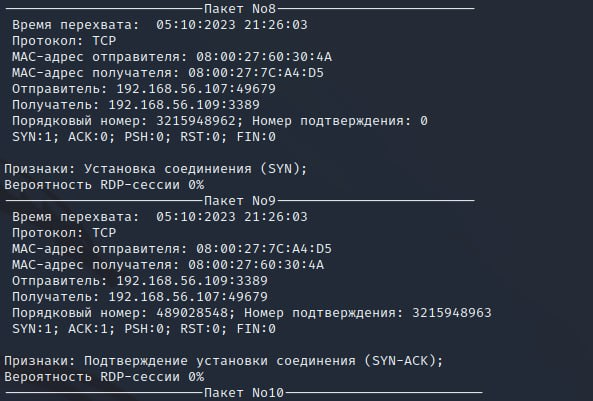
\includegraphics[width=0.7\textwidth]{photo/ses-syn.jpg}
  \caption{Сообщение о перехвате пакета с установлением нового TCP-соединения}
  \label{ses-syn}
\end{figure}


Когда запрос на установку соединения получен и подтвержден, программа ищет TCP-пакет с sequence number, равным acknowledgment number, 
сохраненному на предыдущем этапе, и acknowledgment number текущего пакета, равным sequence number + 1, сохраненному также на предыдущем 
этапе. Это действие означает, что инициатор подключения готов к соединению, и можно считать, что соединение установлено.


Когда обе стороны передали все необходимые данные и произошел обмен подтверждениями о получении последних пакетов данных, TCP-соединение считается 
завершенным. В таких пакетах обычно устанавливается флаг завершения FIN и флаг подтверждения ACK. Если в пакетах установлен флаг сброса RST и флаг 
подтверждения ACK, то TCP-соединение также может быть прервано. При прохождении по всем незавершенным сессиям, если программа <<traffic-detection.py>> 
находит такой пакет, в котором помимо установленного флага подтверждения ACK установлен либо флаг FIN, либо флаг RST, то она считает текущую сессию 
завершенной и рассчитывает общее время данной сессии. Если сессия продлилась менее 10 секунд, она удаляется из списка \textit{Session\_list}. В противном 
случае она остается в списке для дальнейшего анализа трафика.

На рисунках \ref{ses-fin}-\ref{ses-rst} изображены перехваченной программой пакеты, уведомляющие целевое устройство о завершении 
или прерывании активной сессии.

\begin{figure}[H]
  \centering
  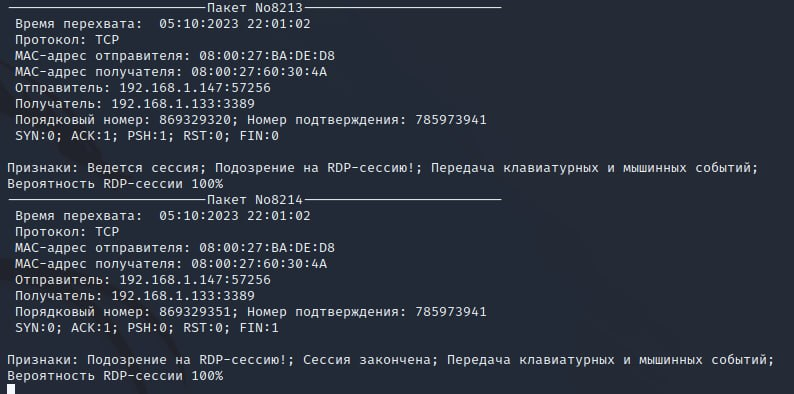
\includegraphics[width=0.7\textwidth]{photo/ses-fin.jpg}
  \caption{Перехват пакета с установленным FIN-флагом}
  \label{ses-fin}
\end{figure}


\begin{figure}[H]
  \centering
  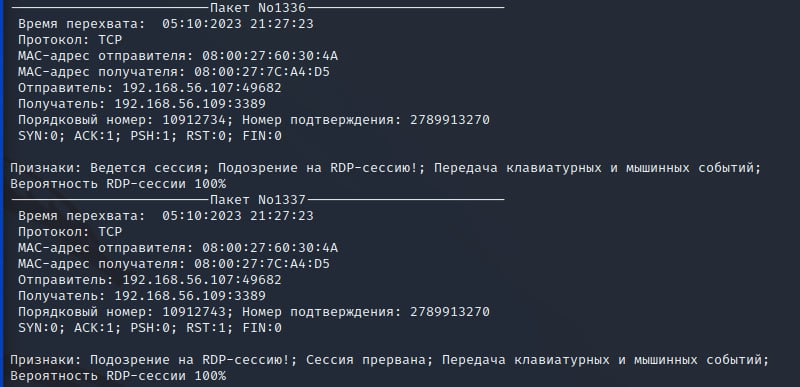
\includegraphics[width=0.7\textwidth]{photo/ses-rst.jpg}
  \caption{Перехват пакета с установленным RST-флагом}
  \label{ses-rst}
\end{figure}

На рисунках помимо признаков TCP-соединения также отображаются некоторые сообщения, связанные с RDP-сессией. 
Подробнее об этих сообщениях будет рассказано в следующих разделах. Однако перед этим необходимо изучить 
проблему выявления признаков протокола RDP.

\subsection{Обработка данных и построение графиков для анализа поведения RDP-трафика}

Тестирование программы происходило на нескольких виртуальных машинах (ВМ), имеющие разные операционные системы.
Использовались операционные системы Windows 10 Professional версии 21H2 и Kali Linux 2022.4 Release. В дальнейшем данные 
операционные системы будем обозначать как Win и Kali соответственно. В эксперименте всегда принимали уачстие три виртуальные машины.
Программа <<traffic-detection.py>> запускалась на третьей ВМ, а между первыми двумя ВМ устанавливалось соединение по протоколу RDP.

Рассматривались следующие соединения:

\begin{itemize}
  \item Соединение Win - Win: устанавливалось соединение между двумя ВМ Windows 10 с помощью приложения
  <<Подключение к удаленному рабочему столу>>; 
  \item Соединение Win - Kali: производилось подключение к Kali LInux с помощью приложения <<Подключение к удаленному рабочему столу>>.
  Для осуществления такого подключения на Kali Linux запускался сервис XRDP, бесплатный протокол удаленного доступа, основанный на 
  протоколе RDP (Microsoft Remote Desktop);
  \item Соединение Kali - Win: для подключения к Windows 10 был использован клиент удаленного рабочего стола Remmina.;
  \item Соединение Kali - Kali: подключение к Kali Linux совершалось с помощью клиента удаленного рабочего стола Remmina.
\end{itemize}

Это было сделано для того, чтобы проанализировать процесс подключения по протоколу RDP между различными операционными системами. Ведь при 
реальной атаке вероятность того, что операционные системы будут одинаковыми, крайне мала. Далее будут рассмотрены статистические методы 
анализа сетевого трафика, которые были выявлены в результате анализа данных различных типов соединений.

\section{Анализ распределения размера пакетов}

Размеры пакетов RDP-трафика обычно больше, чем у других типов трафика, что может быть использовано для обнаружения RDP-сессий. 
Однако, необходимо учитывать, что размеры пакетов могут варьироваться в зависимости от многих 
факторов, таких как тип передаваемой информации, настройки сети и протокола передачи, а также 
особенности конфигурации клиента и сервера RDP.

Тем не менее, можно предположить, что большинство пакетов RDP будут иметь относительно постоянный размер в 
течение сессии, особенно для передачи графических данных. Это может быть использовано для определения наличия активной RDP-сессии.

Например, можно рассчитать средний размер пакета для определенного временного интервала и определить, отличается 
ли этот размер от среднего значения для других протоколов. Также можно рассчитать стандартное отклонение размеров 
пакетов и определить, есть ли значительные отклонения от этого значения для определенного интервала времени, что 
может указывать на активную RDP-сессию.

Однако, стоит отметить, что использование только распределения размеров пакетов не может дать полной уверенности в том, 
что происходит передача RDP-трафика, так как размеры пакетов могут быть изменены в разных версиях протокола, и могут 
использоваться другими протоколами с похожими размерами пакетов. Поэтому, рекомендуется использовать этот метод в 
сочетании с другими методами обнаружения RDP-трафика.


\subsection{Вычисление среднего значения и стандартного отклонения размеров пакетов}

Программа <<traffic-detection.py>> анализирует все активные сессии каждые 5 секунд. В каждом таком интервале времени 
вычисляется среднее значение размера пакетов по формуле:

\begin{center}
  $\mu = \frac{1}{n}\sum_{i = 1}^{n} p_{s_i}$,
\end{center}

где $n$ --- количество пакетов, перехваченных за интервал времени в 5 секунд, $p_{s_i}$ ($1 \leq i \leq n$) --- размер каждого пакета.

Для расчета стандартного отклонения размеров пакетов была использована следующая формула:

\begin{center}
  $\sigma = \sqrt{\frac{1}{n} \sum_{i = 1}^{n} (p_{s_i} - \mu)^2}$,
\end{center}

где $n$ --- количество пакетов,  $p_{s_i}$ ($1 \leq i \leq n$) --- размер каждого пакета, 
$\mu$ --- среднее значение размеров пакетов.

\subsection{Определение верхней и нижней границ диапазона значений размеров пакетов для каждого интервала времени}

Рассчитав среднее значение и стандартное отклонение в пятисекундный интервал времени, программа делает следующие операции:

\begin{enumerate}
  \item Производится определение верхней (ВГ) и нижней (НГ) границы диапазона значений размеров пакетов, в котором должно находиться 
  большинство пакетов для этого интервала времени. Эти границы могут быть определены путем добавления или вычитания отклонения 
  от среднего значения размеров пакетов, к верхней или нижней границе. В данном случае  НГ $= (\mu - 4\sigma)$ и ВГ $= (\mu + 4\sigma)$.
  \item Проверяется каждый размер пакета в интервале времени на соответствие этим границам. 
  Если размер пакета выходит за пределы этого диапазона значений ($p_{s_i} < (\mu - 4\sigma)$ или $p_{s_i} > (\mu + 4\sigma)$ ($1 \leq i \leq n$)), 
  то это может указывать на наличие активной RDP-сессии.
  \item Программа определяет наличие пакетов с аномальными размерами, характерными для признаков RDP-сессии, на основе того, удовлетворяют ли более 60\% 
  перехваченных пакетов вышеописанным условиям в определенном интервале времени.
\end{enumerate}

\subsection{Анализ полученных данных на наличие признаков RDP-сессии}

Стоит отметить, что выбор коэффициента, множителя для стандартного отклонения, выбирался, на основе соединений, в каждом из которых производилась 
установка RDP-сессии.

График на рисунке \ref{win-size} отображает максимальное значение пакетов, рассчитанных за единицу времени, при использовании соединения Win-Win. 
На этом графике представлены только максимальные значения, которые были рассчитаны на основе пакетов, относящихся к протоколу RDP. По этому 
графику можно сделать несколько выводов:


\begin{figure}[H]
  \centering
  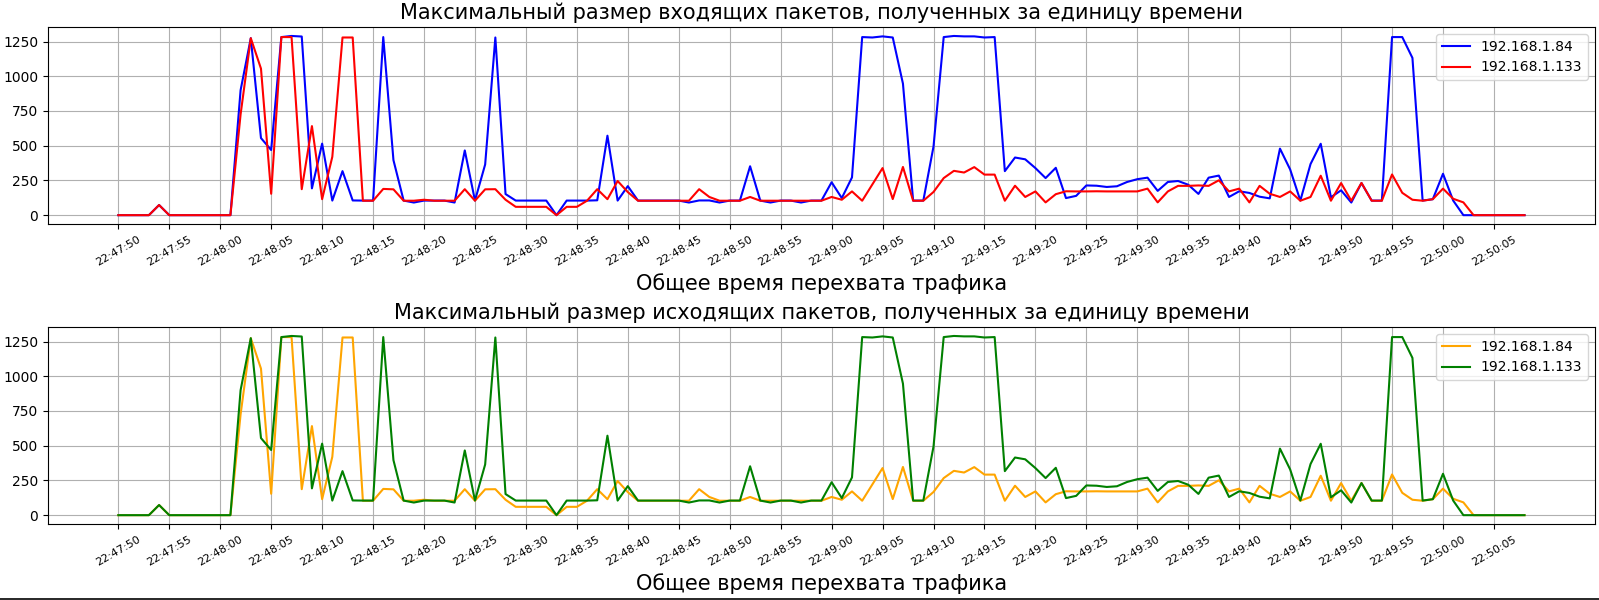
\includegraphics[width=0.8\textwidth]{photo/size-win.png}
  \caption{График отображения максимумов среди пакетов, рассчитанных в единицу времени (соединение Win - Win)}
  \label{win-size}
\end{figure}


\begin{itemize}
  \item максимальный размер таких пакетов не превышает 1300 байт; 
  \item Обычно, по количеству пакетов, переданных между устройствами, можно определить инициатора подключения и целевое 
  устройство. В данном случае инициатором подключения является устройство с IP-адресом 192.168.1.84, а целевым устройством - 
  устройство с IP-адресом 192.168.1.133, так как первое получило большее количество пакетов с максимальными размерами байт;
  \item В промежуток времени между 22:48:00 и 22:48:15 размеры пакетов инициатора подключения и целевого устройства достигают 
  максимального размера байт в тот момент, когда происходит этап процесса аутентификации и защиты передаваемых данных (обмен сертификатами). 
  Этот этап происходит в начале установления соединения и позволяет клиенту и серверу проверить 
  подлинность друг друга и договориться о параметрах безопасности соединения.
  Такой обмен, когда размеры пакетов целевого устройства достигают максимума, заметен только при 
  подключении между двумя ВМ Windows 10.
\end{itemize}

Также можно сделать аналогичные выводы по остальным соединениям из рисунков \ref{winkal-size} - \ref{kali-size}. 
Графики показывают, что максимальные размеры пакетов в других соединениях значительно отличаются от соединения 
Win - Win. Кроме того, в момент, когда происходит этап процесса аутентификации и защиты передаваемых данных, 
не наблюдается такого явного обмена пакетами.


\begin{figure}[H]
  \centering
  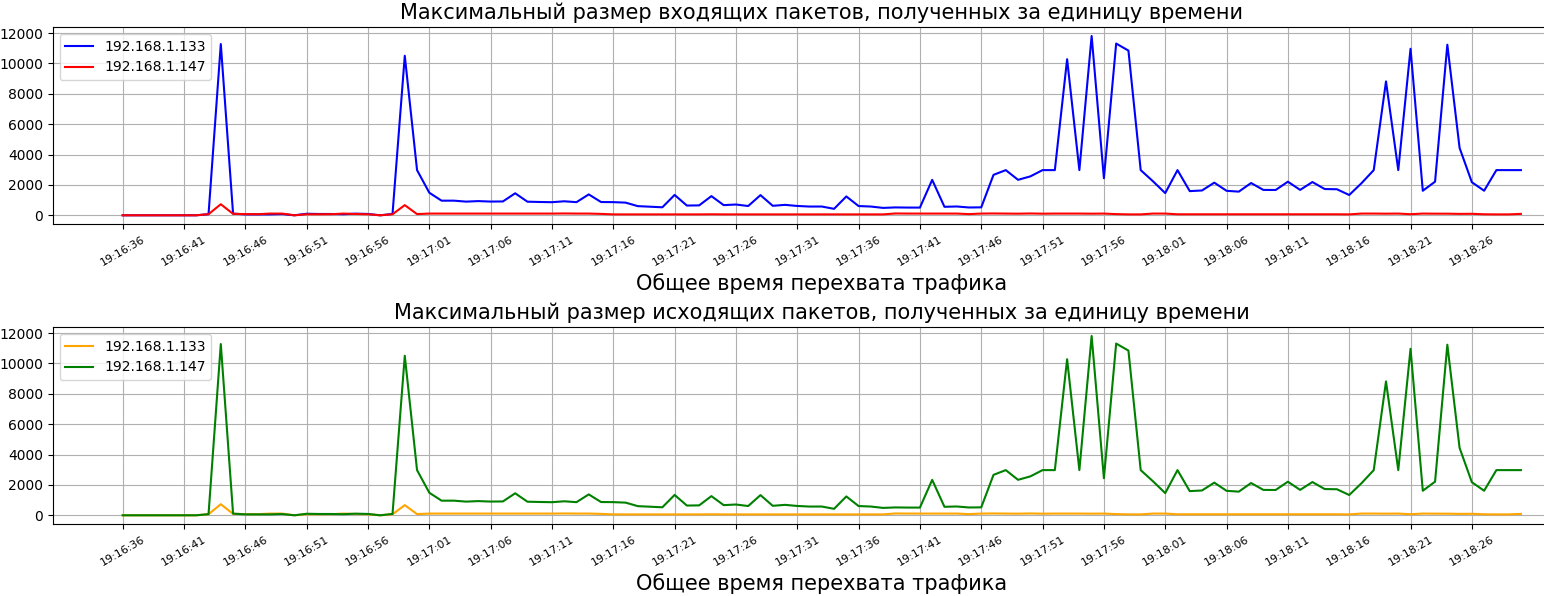
\includegraphics[width=0.8\textwidth]{photo/size-winkal.png}
  \caption{График отображения максимумов среди пакетов в единицу времени (соединение Win - Kali)}
  \label{winkal-size}
\end{figure}


\begin{figure}[H]
  \centering
  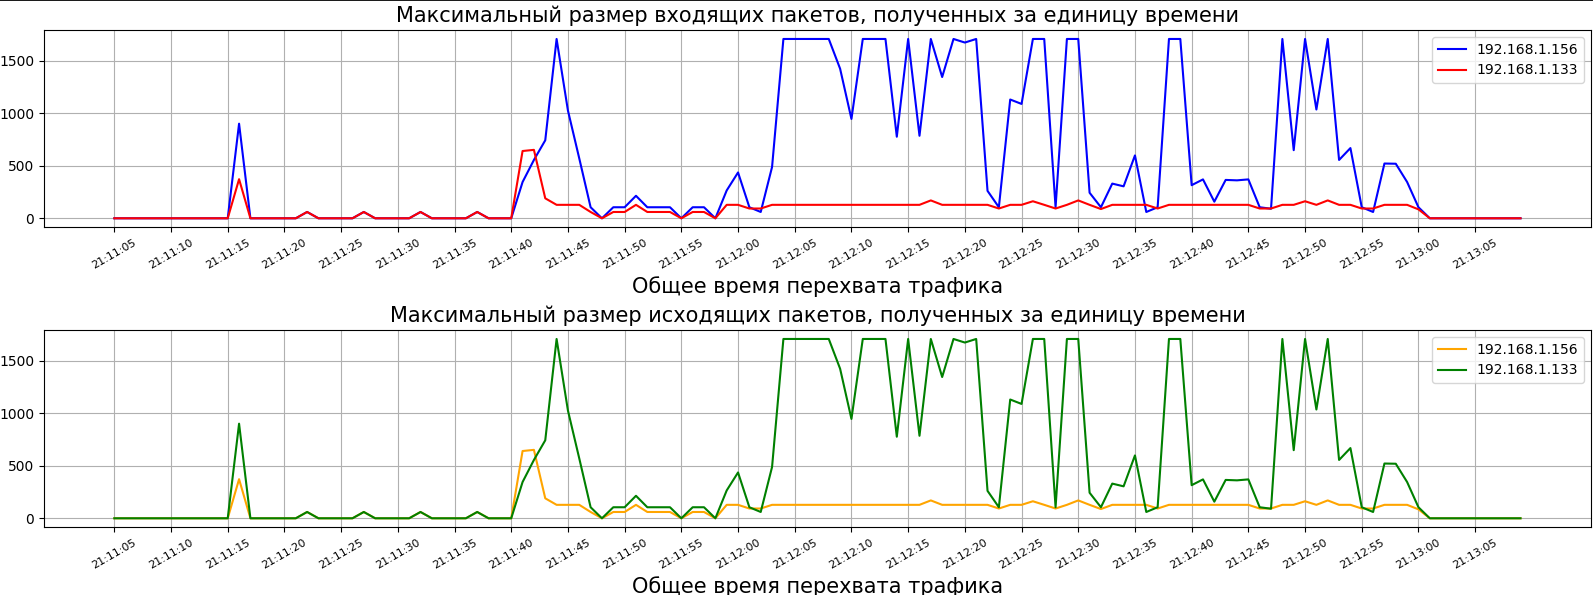
\includegraphics[width=0.8\textwidth]{photo/size-kalwin.png}
  \caption{График отображения максимумов среди пакетов в единицу времени (соединение Kali - Win)}
  \label{kalwin-size}
\end{figure}


\begin{figure}[H]
  \centering
  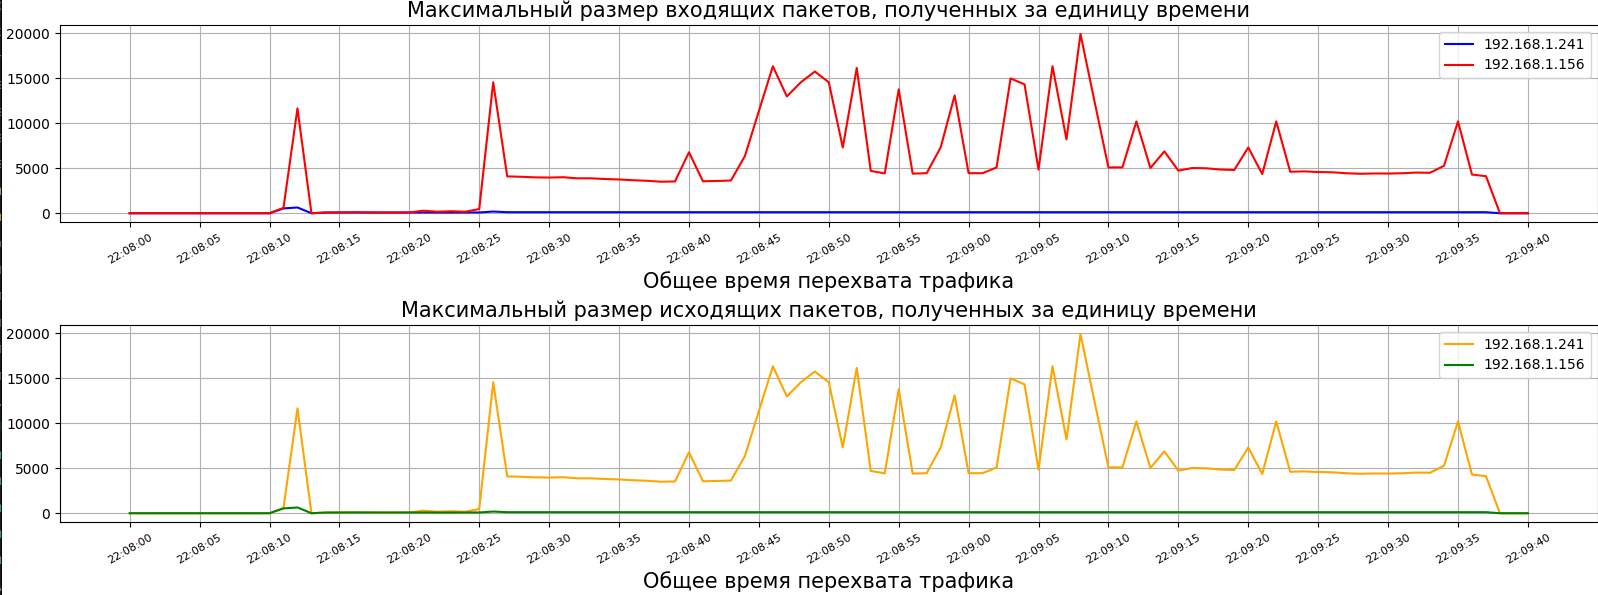
\includegraphics[width=0.8\textwidth]{photo/size-kal.png}
  \caption{График отображения максимумов среди пакетов в единицу времени (соединение Kali - Kali)}
  \label{kali-size}
\end{figure}

На следующем рисунке показано одно из подключений по SSH, в котором можно заметить аномальные размеры
пакетов только в самом начале подключения. В последующих интервалах времени размеры пакетов не выходят за пределы 
НГ и ВГ, поэтому программе в данном случае удается различить протоколы RDP и SSH.


\begin{figure}[H]
  \centering
  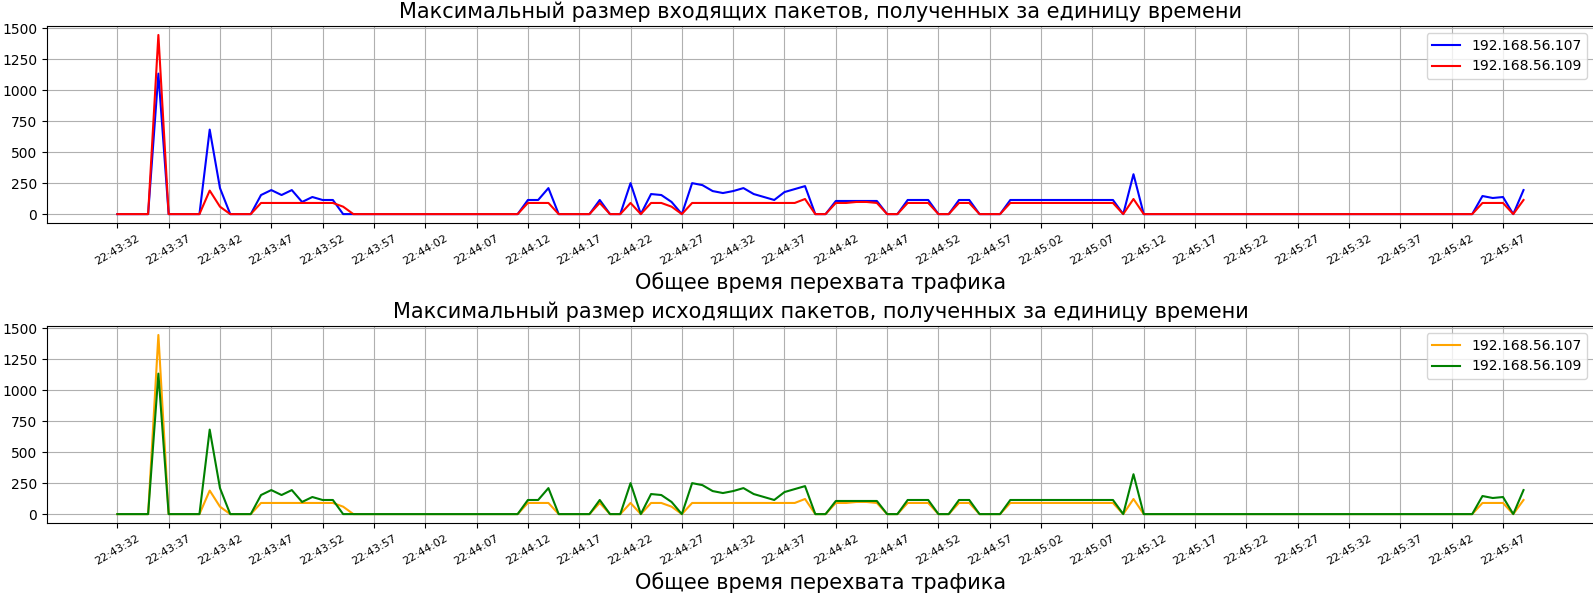
\includegraphics[width=0.8\textwidth]{photo/size-ssh.png}
  \caption{График отображения максимумов среди пакетов в единицу времени (подключение по SSH)}
  \label{ssh-size}
\end{figure}


Исходя из вышеописанных рассуждений, именно таким образом программа <<traffic-detection.py>> 
проводит анализ распределения пакетов.


\section{Анализ распределения временных интервалов между пакетами}

Анализ распределения временных интервалов между пакетами может быть полезен для обнаружения RDP-сессий. 
Обычно временные интервалы между пакетами RDP-трафика меньше, чем между пакетами других типов трафика. 
Это связано с тем, что RDP-протокол предназначен для передачи данных в режиме реального времени и требует 
высокой скорости передачи данных для обеспечения плавной работы удаленного рабочего стола. Поэтому, если 
на сети обнаруживается высокая частота пакетов с маленькими временными интервалами, это может быть признаком 
активной RDP-сессии. Однако следует учитывать, что также могут быть и другие типы трафика, которые также используют 
высокую скорость передачи данных и могут иметь маленькие временные интервалы между пакетами, поэтому этот метод должен 
использоваться вместе с другими методами обнаружения RDP-трафика.
 
\subsection{Вычисление среднего значения и стандартного отклонения интервалов}
Расчет временных интервалов программа <<traffic-detection.py>> делает для каждой активной сессии. Она запоминает время предыдущего пакета $t_{prev}$ и 
находит разность текущего ($t_{cur}$) перехваченного пакета и предыдущего ($t_{cur} - t_{prev}$). Каждые пять секунд программа вычисляет 
среднее значение интервалов времени по формуле:

\begin{center}
  $\mu = \frac{1}{n}\sum_{i = 1}^{n - 1} t_{i}$,
\end{center}

где $n$ --- количество пакетов, перехваченных за интервал времени в 5 секунд, $t_i$ ($1 \leq i \leq n - 1$) --- интервал времени между двумя 
последовательно идущими пакетами.

Для расчета стандартного отклонения размеров пакетов была использована следующая формула:

\begin{center}
  $\sigma = \sqrt{\frac{1}{n - 1} \sum_{i = 1}^{n - 1} (t_{i} - \mu)^2}$,
\end{center}

где $n$ --- количество пакетов, перехваченных за интервал времени в 5 секунд, $t_i$ ($1 \leq i \leq n - 1$) --- интервал времени между двумя 
последовательно идущими пакетами, 
$\mu$ --- среднее значение интервалов времени.

\subsection{Определение пороговых значений для интервалов}


После того как были рассчитаны среднее значение и стандартное отклонение в пятисекундный интервал времени, программа производит следующие операции:

\begin{enumerate}
  \item Для определения верхней (ВГ) и нижней (НГ) границ диапазона значений временных интервалов пакетов используется метод добавления или 
  вычитания отклонения от среднего значения интервалов времени к верхней или нижней границе. В данном случае, НГ и ВГ определяются как 
  НГ $= (\mu - \frac{5}{9}\sigma)$ и ВГ $= (\mu + \frac{5}{9}\sigma)$. 
  \item В пятисекундном интервале времени проверяется каждый $t_i (1 \leq i \leq n - 1)$ на соответствие этим границам. 
  Если некоторый интервал времени выходит за пределы этого диапазона значений ($t_i < (\mu - \frac{5}{9}\sigma)$ или $t_i > (\mu - \frac{5}{9}\sigma)$ 
  ($1 \leq i \leq n - 1$)), то это может указывать на наличие активной RDP-сессии.
  \item Программа определяет наличие пакетов с аномальными временными интервалами, характерными для признаков RDP-сессии, на основе того, 
  удовлетворяют ли более 50\% перехваченных пакетов вышеописанным условиям в определенном интервале времени.
\end{enumerate}

\subsection{Анализ полученных данных на наличие признаков RDP-сессии}

Важно отметить, что выбор коэффициента $\frac{5}{9}$, множителя для стандартного отклонения, был сделан на основе соединений, 
в каждом из которых была установлена RDP-сессия. В большинстве случаев стандартное отклонение оказывалось больше среднего значения интервалов времени. 
Это означает, что значения разбросаны вокруг среднего значения более широко, чем при более низком стандартном отклонении. Почти все интервалы времени 
выходили за пределы значений НГ и ВГ. После небольшого подбора был найден коэффициент, равный $\frac{5}{9}$, который позволил программе во всех
типах соединения обнаруживать маленькие временные интервалы, которые могут быть признаками RDP-сессии.


Однако нельзя полностью полагаться на данный метод, так как высокая частота пакетов может также являться признаком каких-либо других протоколов, например,
HTTP или HTTPS. Поэтому рассматривать его отдельно не имеет смысла. 


\section{Анализ частоты флагов PSH}


Флаг PSH (Push) используется в протоколах удаленного рабочего стола, включая RDP и VNC. 
Этот флаг устанавливается в TCP-заголовке и сообщает получающей стороне, что передаваемые данные должны 
быть немедленно переданы приложению-получателю без буферизации на стороне получателя. Флаг PSH часто 
используется в протоколах, которые используют потоковую передачу данных, таких как терминальные протоколы 
или удаленный рабочий стол, чтобы уменьшить задержки в передаче данных и улучшить отзывчивость приложения.

В протоколе RDP флаг PSH может использоваться для передачи клавиатурных и мышиных событий с клиента на сервер, 
а также для отправки команд и получения ответов на них. Он также может использоваться для передачи буферизованных 
изображений и звуковых данных. 

Таким образом, рассчитывая частоту флагов PSH в каждом интервале времени можно обнаружить RDP-сессии. 

\subsection{Расчет частоты флагов PSH для каждого интервала времени}

Каждые 5 секунд, программа считает TCP-пакеты и TCP-пакеты с установленным флагом PSH. По завершении
5 секунд были получены две величины: $V_{P_{in}}$ --- объем входящего трафика с установленным флагом PSH и $V_{tcp}$ --- число входящих
TCP-пакетов в пятисекундный интервал времени.

Таким образом, частота PSH-флагов равна:
\begin{center}
  $r_{psh} = \frac{V_{P_{in}}}{V_{tcp}}$
\end{center} 

Вместе с этим программа смотрит на значения частоты PSH-флагов, рассчитанные в предыдущие интервалы времени. Посчитав их среднее значение $\mu_{psh}$,
программа проверяет следующие условия: если $cur_{psh} > 0$ и $| \mu_{psh} - cur_{psh}| < 0.3$, где $cur_{psh}$ --- текущий интервал времени, то 
в данный момент совершаются клавиатурные или мышиные события.


\subsection{Анализ полученных данных на наличие признаков RDP-сессии}

Просматривая каждый TCP-пакет, программа проверяет наличие установленного флага PSH в тех пакетах, где IP-адрес 
получателя является целевым устройством. Т.е. программа пытается анализировать тот момент, когда инициатор подключения
отправляет TCP-пакеты с установленным PSH-флагом.


На рисунках \ref{win-psh} - \ref{kali-psh} показаны графики, на которых изображена частота PSH-флагов при установке RDP-сессии 
в различных типах соединения. В данном случае инициаторами подключения являются устройства, показанные желтым цветом, а целевые устройства --- 
зеленым цветом. Главной задачей программы являлось нахождение таких интервалов времени в которых среднее значение частоты флагов будет примерно
одинаково и больше нуля.

\begin{figure}[H]
  \centering
  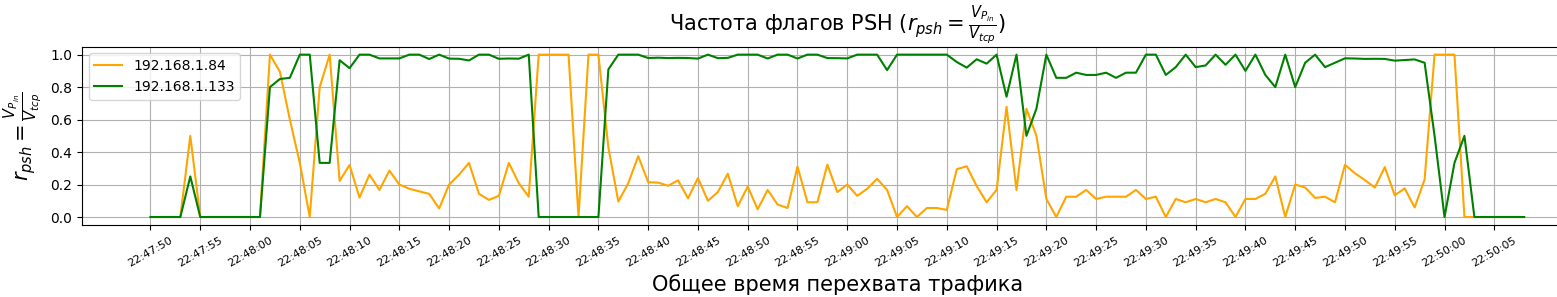
\includegraphics[width=0.8\textwidth]{photo/psh-win.png}
  \caption{График частоты PSH флагов (соединение Win - Win)}
  \label{win-psh}
\end{figure}

На примере рисунка \ref{winkal-psh} можно легко увидеть, когда пользователь взаимодействовал с мышью или клавиатурой, а когда оставался 
бездействующим. Например, на промежутке между 19:17:16 и 19:17:37 не было зафиксировано движений мыши или нажатий клавиш на клавиатуре, 
тогда как на остальных временных отрезках пользователь совершал какие-либо действия. Таким образом, если в определенный момент времени 
частота PSH-флагов равна нулю, можно сделать вывод, что в это время никаких действий не происходило.

\begin{figure}[H]
  \centering
  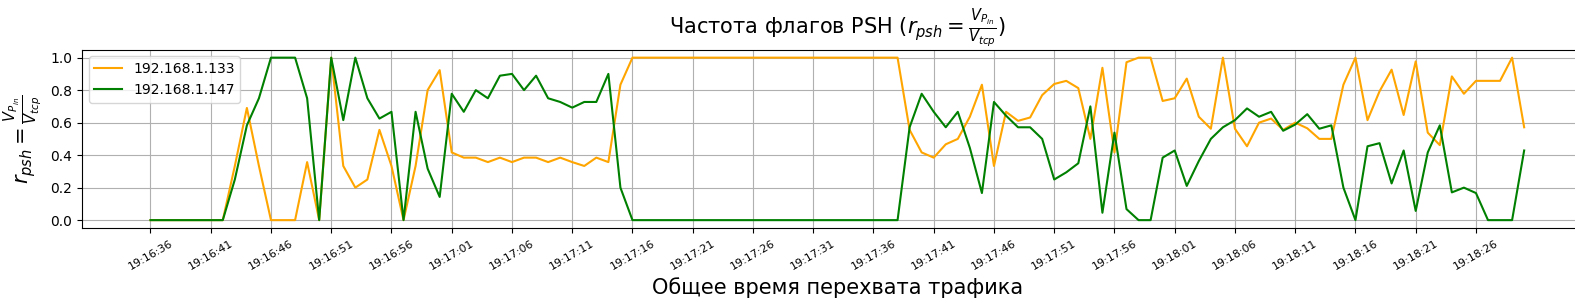
\includegraphics[width=0.8\textwidth]{photo/psh-winkal.png}
  \caption{График частоты PSH флагов (соединение Win - Kali)}
  \label{winkal-psh}
\end{figure}


\begin{figure}[H]
  \centering
  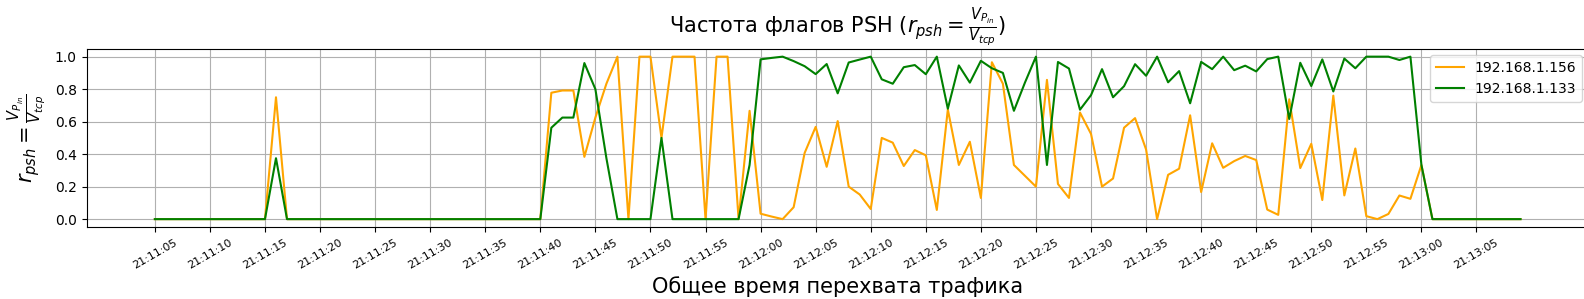
\includegraphics[width=0.8\textwidth]{photo/psh-kalwin.png}
  \caption{График частоты PSH флагов (соединение Kali - Win)}
  \label{kalwin-psh}
\end{figure}

Однако, при соединении двух ВМ Kali программа будет выдавать ложные срабатывания в момент бездействия пользователя. На промежутке времени
между 22:08:25 и 22:08:40 пользователь не совершал никаких действий при активной RDP-сессии, и из рисунка \ref{kali-psh} видно, что частота флагов
PSH не равна нулю. В этом временном интервале передается фиксированное количество PSH-флагов. 

\begin{figure}[H]
  \centering
  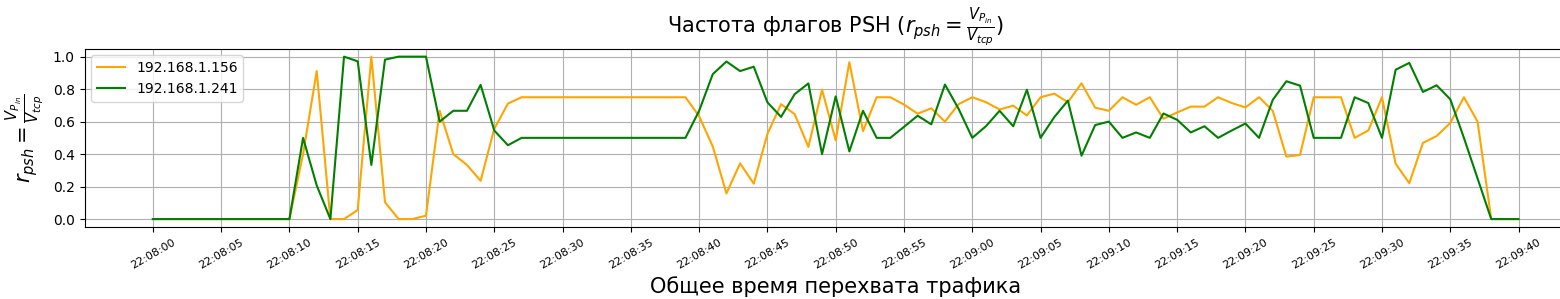
\includegraphics[width=0.8\textwidth]{photo/psh-kal.png}
  \caption{График частоты PSH флагов (соединение Kali - Kali)}
  \label{kali-psh}
\end{figure}

В данном случае из-за такой особенности типа соединения Kali - Kali программа <<traffic-detection.py>> не сможет точно определить 
взаимодействия с мышью и клавиатурой.



\section{Некоторые модификации для улучшения обнаружения RDP-сессии}


Стоит отметить, что из вышеописанных статистических методов анализа сетевого трафика самым ненадежным оказался анализ временных интервалов между пакетами.
Данный метод постоянно выдавал ложные срабатывания, так как программа находила маленькие интервалы времени в других протоколах, не похожих на RDP. 
После целого ряда различных тестирований была придумана небольшая модификация, которая должна работать в совокупности с этим ненадежным методом.
Она заключается в нахождении отношения объема входящего трафика и исходящего трафика в единицу времени. 

На рисунках \ref{win-inout} - \ref{kali-inout} показаны графики отношения входящего и исходящего трафика, рассчитанные
при активной RDP-сессии в четырех типах соединения. Инициаторами подключения являются устройства, показанные синим цветом, 
а целевые устройства --- оранжевым цветом.


\begin{figure}[H]
  \centering
  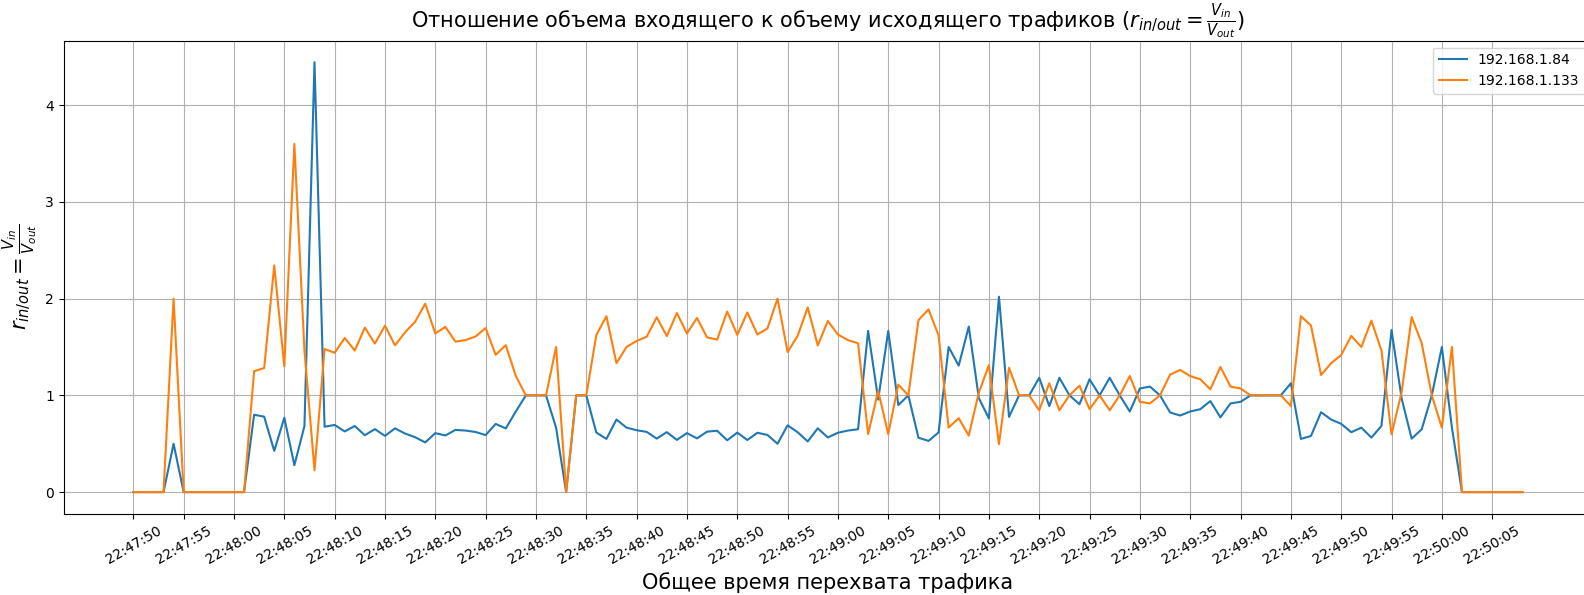
\includegraphics[width=0.8\textwidth]{photo/inout-win.png}
  \caption{График отношения объема входящего и исходящего трафика (соединение Win - Win)}
  \label{win-inout}
\end{figure}


\begin{figure}[H]
  \centering
  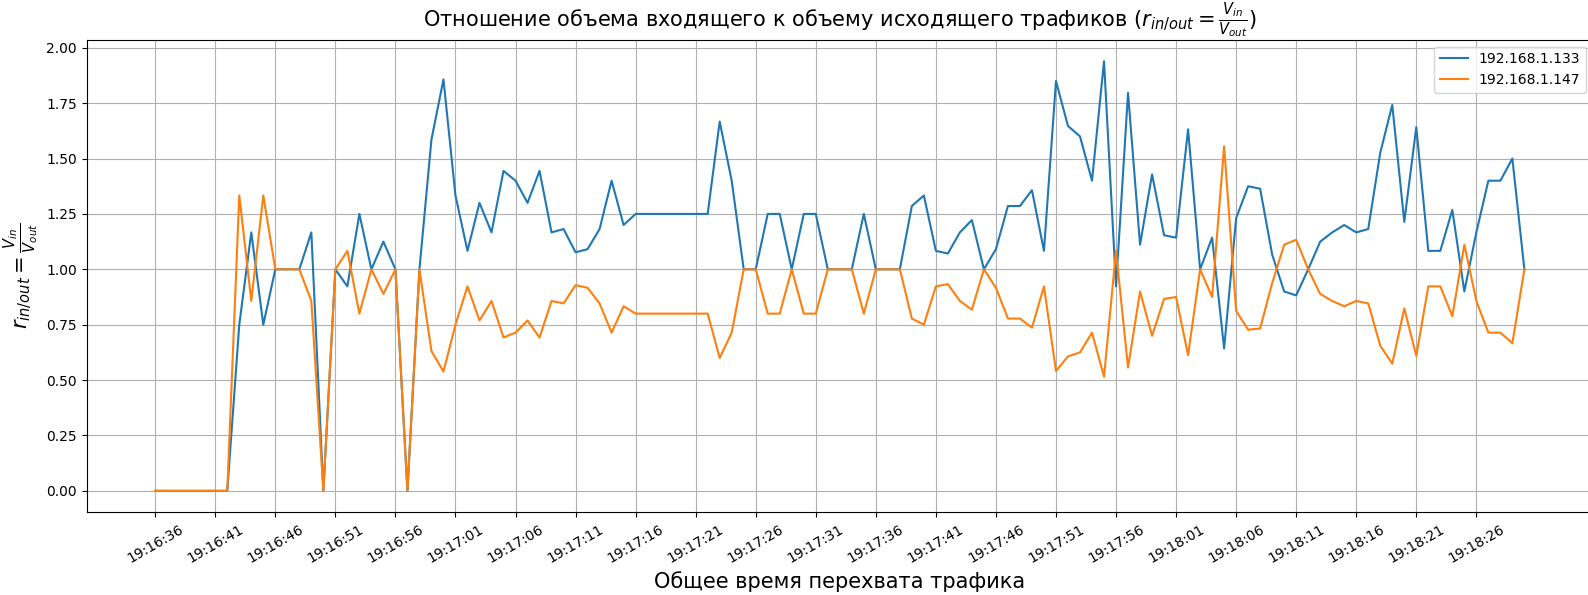
\includegraphics[width=0.8\textwidth]{photo/inout-winkal.png}
  \caption{График отношения объема входящего и исходящего трафика (соединение Win - Kali)}
  \label{winkal-inout}
\end{figure}

% Стоит отметить, что при подключении к ВМ Windows 10 по протоколу RDP целевое устройство получает
% больше пакетов чем инициатор подключения. А при подключении к ВМ Kali всё наоборот. Есть предположение, что
% различное количество пакетов, передаваемых при соединении по протоколу RDP между Windows и Linux, 
% может быть связано с различиями в реализации протокола на этих операционных системах. Поэтому скорее всего
% если выполнить в ВМ Windows конкретные настройки, то количество передаваемых пакетов может измениться. 


\begin{figure}[H]
  \centering
  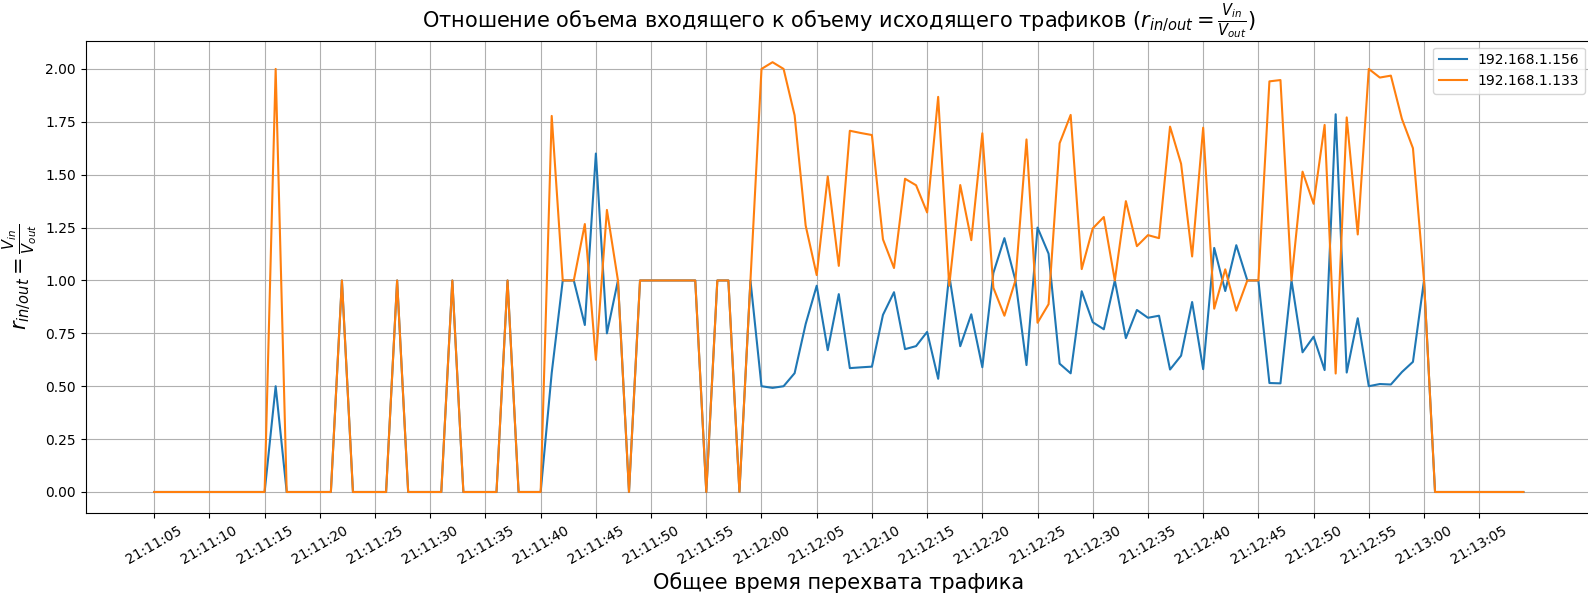
\includegraphics[width=0.8\textwidth]{photo/inout-kalwin.png}
  \caption{График отношения объема входящего и исходящего трафика (соединение Kali - Win)}
  \label{kalwin-inout}
\end{figure}


\begin{figure}[H]
  \centering
  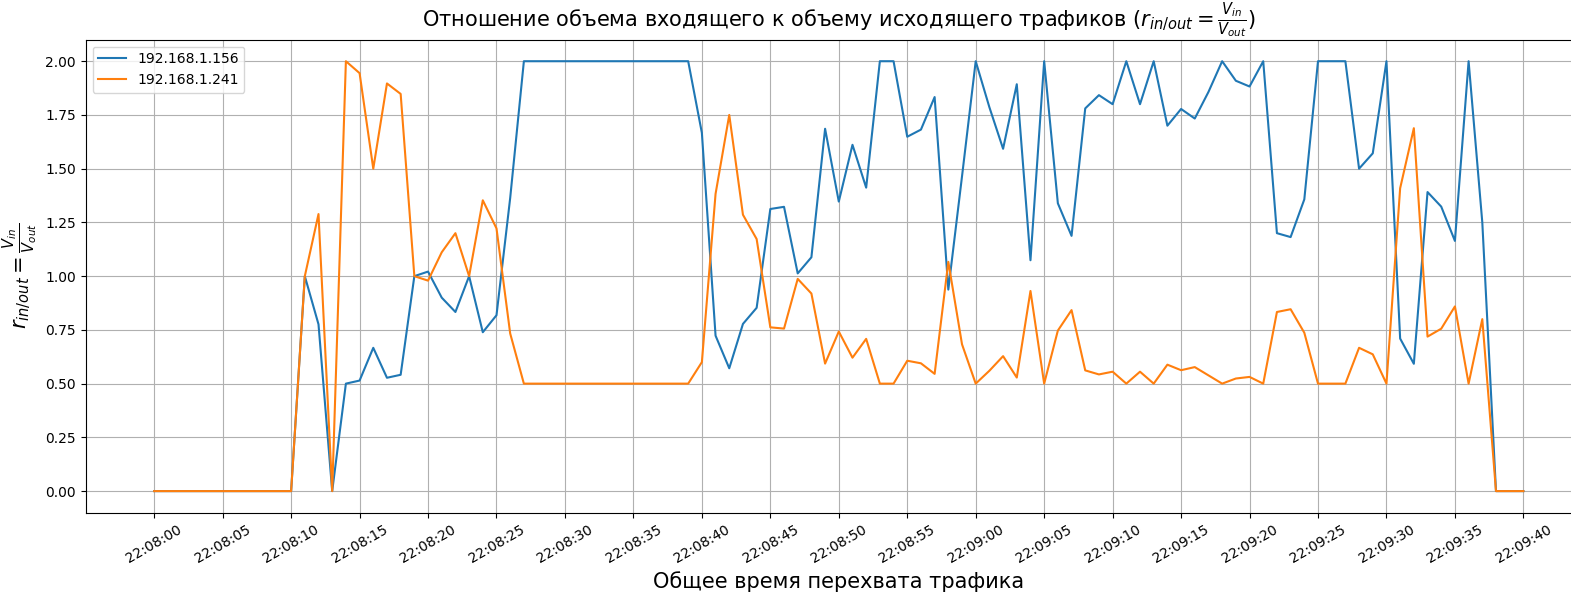
\includegraphics[width=0.8\textwidth]{photo/inout-kali.png}
  \caption{График отношения объема входящего и исходящего трафика (соединение Kali - Kali)}
  \label{kali-inout}
\end{figure}

Как можно заметить из рисунков \ref{win-inout} - \ref{kali-inout}, то значения отношения входящего и исходящего трафика
при активной RDP-сессии находятся в основном между 0.5 и 2.0. Конечно, нельзя однозначно утверждать, что такой диапазон
значений характерен только для протокола RDP, например, на следующем рисунке показан график отношения объема входящего и
исходящего трафиков при активной SSH-сессии. Из рисунка \ref{ssh-inout}
видно, что в некоторые промежутки времени значения попадают в промежуток [0.5, 2.0]. Однако, метод анализа временных интервалов между пакетами
в этом случае не будет реагировать на данные значения так как при подключении по SSH наблюдается низкая скорость передачи пакетов,
и программа <<traffic-detection.py>> посчитает, что здесь нет никаких признаков RDP-сессии.

\begin{figure}[H]
  \centering
  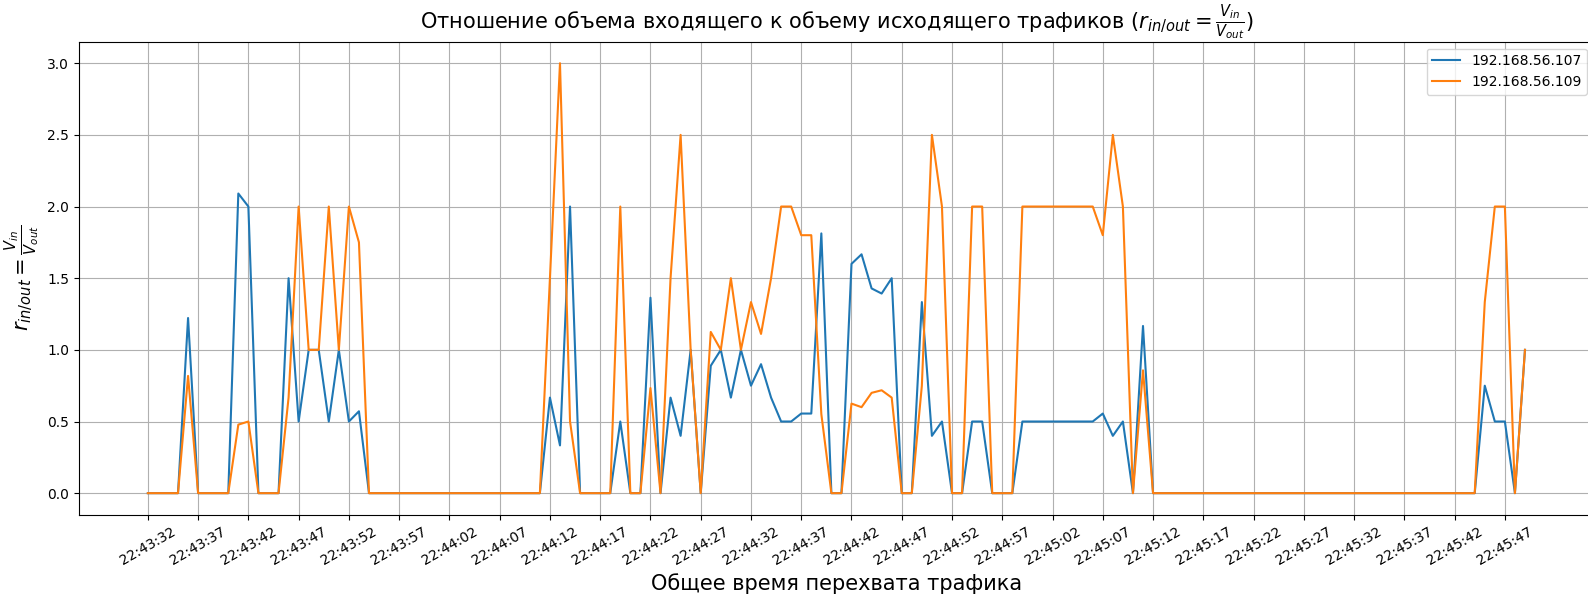
\includegraphics[width=0.8\textwidth]{photo/inout-ssh.png}
  \caption{График отношения объема входящего и исходящего трафика (подключение по SSH)}
  \label{ssh-inout}
\end{figure}

На рисунке изображен график соотношения объема входящего и исходящего HTTP-трафика. 
При использовании метода анализа временных интервалов между пакетами программа <<traffic-detection.py>> 
в некоторых случаях может неправильно интерпретировать временные интервалы и считать их значением, превышающим пороговые значения, 
что может быть ошибочно расценено как признак RDP-сессии, хотя на самом деле происходит перехват HTTP-трафика. Однако в таких 
ситуациях нахождение соотношения входящего и исходящего трафика может помочь различить протоколы RDP, HTTP и HTTPS.

\begin{figure}[H]
  \centering
  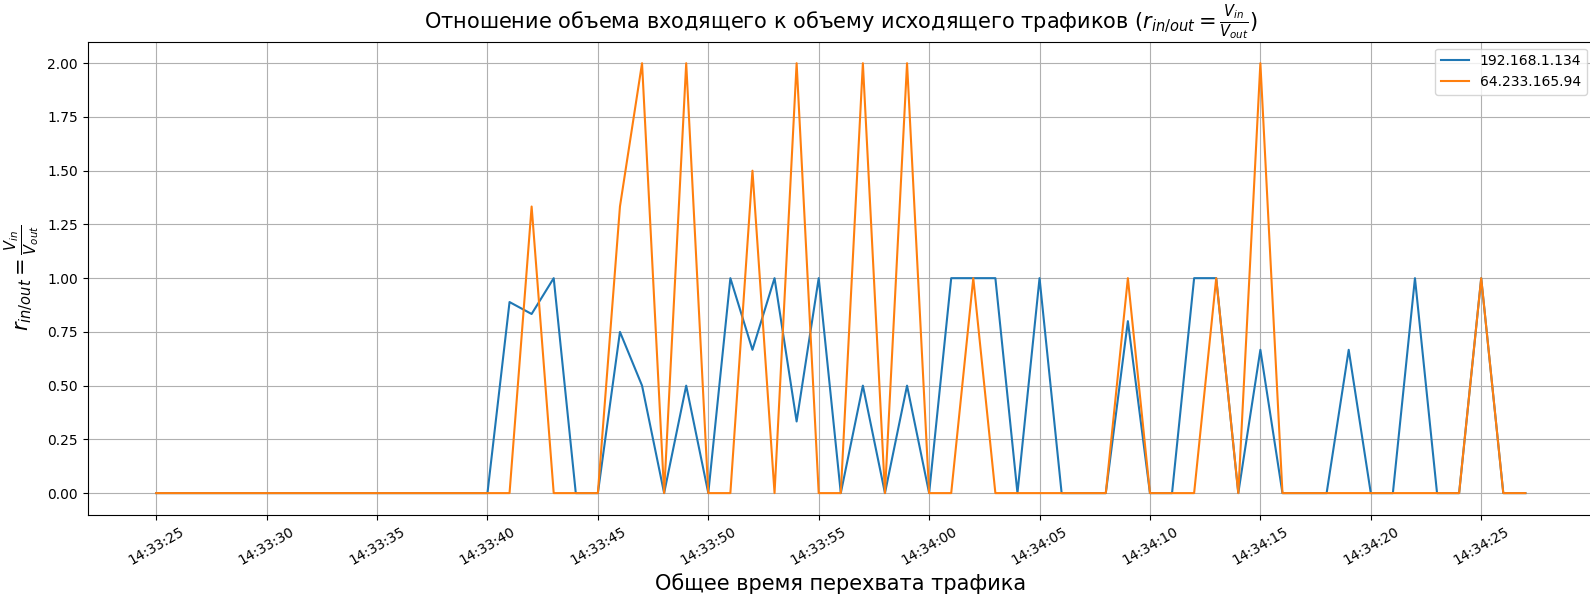
\includegraphics[width=0.8\textwidth]{photo/inout-http.png}
  \caption{График отношения объема входящего и исходящего трафика (подключение по HTTP)}
  \label{http-inout}
\end{figure}

Таким образом отношение входящего к исходящему трафиков дополняет метод анализа временных интервалов между пакетами.

На протяжении всей активной сессии программа <<traffic-detection.py>> считает количество пакетов входящего и исходящего трафика
инициатора подключения и целевого устройства. Когда проходит одна секунда с момента подсчета пакетов, программа находит отношения
по следующим формулам:

\begin{center}
  $r_{init} = \frac{V_{i_{dest}}}{V_{i_{src}}}$,
\end{center}

где $V_{i_{dest}}$ и $V_{i_{src}}$ --- объемы входящего и исходящего трафика инициатора, рассчитанные в единицу времени. 

\begin{center}
  $r_{targ} = \frac{V_{t_{dest}}}{V_{t_{src}}}$,
\end{center}

где $V_{t_{dest}}$ и $V_{t_{src}}$ --- объемы входящего и исходящего трафика целевого устройства, рассчитанные в единицу времени. 

Каждые пять секунд производится анализ состояния сети, где вычисляется средние значения величин $r_{init_{k}}$ и $r_{targ_{k}}$ ($1 \leq k \leq 5$)

\begin{center}
  $\mu_{init} = \frac{1}{5}\sum_{k = 1}^{5} r_{init_{k}}$,
\end{center}

где $r_{init_{k}}$ ($1 \leq k \leq 5$) --- отношения входящего и исходящего трафика инициатора подключения.


\begin{center}
  $\mu_{targ} = \frac{1}{5}\sum_{k = 1}^{5} r_{targ_{k}}$,
\end{center}

где $r_{init_{k}}$ ($1 \leq k \leq 5$) --- отношения входящего и исходящего трафика целевого устройства.

Далее программа проверяет следующее: если значения $\mu_{init} \in (1, 2) $ и $\mu_{targ} \in [0.5, 1)$ или 
$\mu_{targ} \in (1, 2) $ и $\mu_{init} \in [0.5, 1)$, а также $|\mu{init} - \mu{targ}| \in (0.2, 1.8)$, значит 
на данном временном интервале возможно наличие признаков RDP-сессии. 

И если на этом же пятисекундном интервале анализ временных интервалов между пакетами показал положительный результат, то здесь действительно
наблюдается RDP-сессия.


\section{Тестирование программы на определение наличия или отсутствия RDP-сессии}

Тестирование заключалось в том, что запускались три виртуальные машины, на первых двух создавалась активная RDP-сессия,
а на третьей ВМ запускалась программа <<traffic-detection.py>> в режиме перехвата трафика.

На следующем рисунке показано подключение по протоколу RDP при соединении Kali - Win. На ВМ Kali (192.168.1.147) был установлен клиент удаленного
рабочего стола Remmina, с помощью которого было совершено соединение с ВМ Windows 10 (192.168.1.133).

\begin{figure}[H]
  \centering
  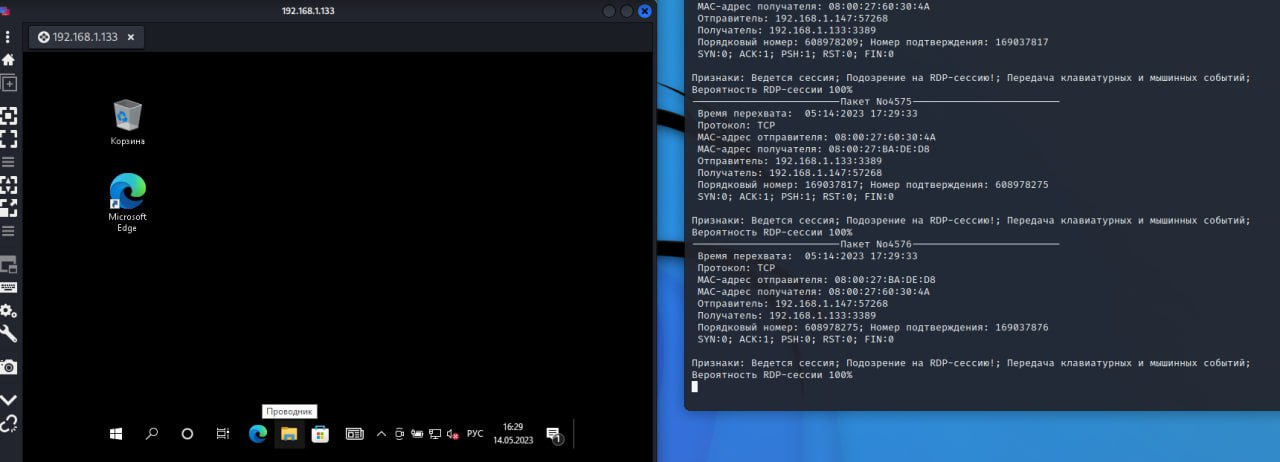
\includegraphics[width=0.8\textwidth]{photo/rdp1.jpg}
  \caption{Работа программы при установке RDP-сессии (соединение Kali - Win) }
  \label{rdp1}
\end{figure}

Из рисунка \ref{rdp1} видно, что подключение совершалось по порту 3389, который используется протоколом RDP по умолчанию, и 
программа смогла однозначно определить наличие в сети активной RDP-сессии. Можно заметить в <<признаках>> сообщение <<Передача клавиатурных и
мышинных событий>>. Это результат работы метода анализа частоты PSH-флагов. В программе вероятность считается исходя из результатов состояния сети,
сделанных на предыдущих временных интервалах относительно данной сессии. Однако здесь очень простой случай, так как программа обнаружила стандартный
RDP-порт. 

Рассмотрим следующий пример, где установка RDP-сессии происходит на другой порт. На рисунке \ref{rdpport1} изображено изменение
значения стандартного RDP-порта на 13389. Это операция делается в редакторе реестра Windows. Информацию о том, как это можно сделать
описана в документации Microsoft \cite{rdpport}.


\begin{figure}[H]
  \centering
  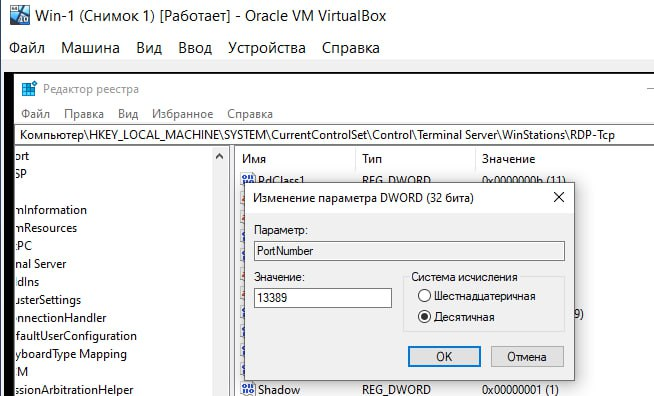
\includegraphics[width=0.8\textwidth]{photo/rdpport1.jpg}
  \caption{Изменение номера порта по умолчанию на порт 13389}
  \label{rdpport1}
\end{figure}

На следующем рисунке показано, что на третьей ВМ был начат перехват трафика с использованием фильтра RDP. Данное условие подразумевает то,
что в консоль будет выводится информация только о тех пакетах которые несут в себе признаки RDP.

\begin{figure}[H]
  \centering
  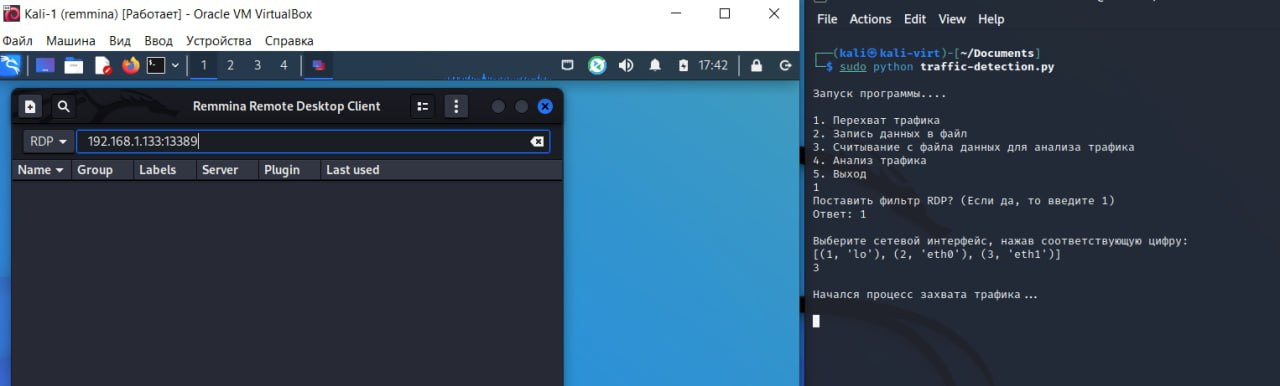
\includegraphics[width=1\textwidth]{photo/rdpport2.jpg}
  \caption{Установка RDP-сессии по порту 13389}
  \label{rdpport2}
\end{figure}

Спустя 25 секунд после установки RDP-сессии программа посчитает количество таких временных интервалов, в которых были найдены
признаки RDP-сессии. Если таких временных интервалов окажется больше 50\%, то программа будет выводить информацию о текущих пакетах.

На рисунке \ref{rdpport3} показана вероятность RDP-сессии на текущий момент времени.

\begin{figure}[H]
  \centering
  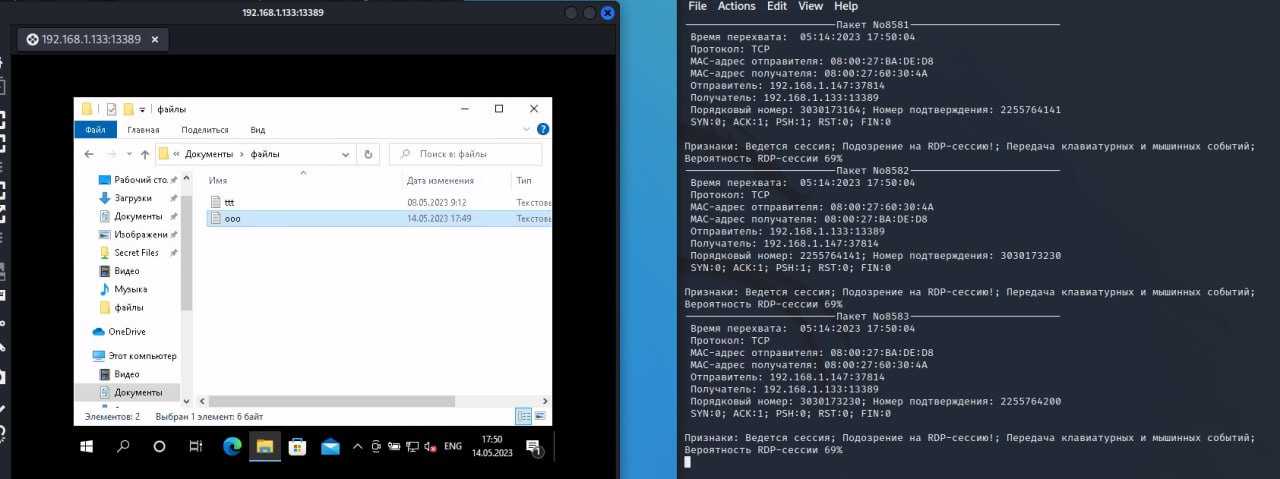
\includegraphics[width=0.8\textwidth]{photo/rdpport3.jpg}
  \caption{Демонстрация работы программы при активной RDP-сессии}
  \label{rdpport3}
\end{figure}

А из следующего рисунка видно, что спустя несколько секунд после установки соединения, вероятность RDP-сессии увеличилась.
Это связано с тем, что за некоторый интервал времени производились взаимодействия с мышкой и клавиатурой.


\begin{figure}[H]
  \centering
  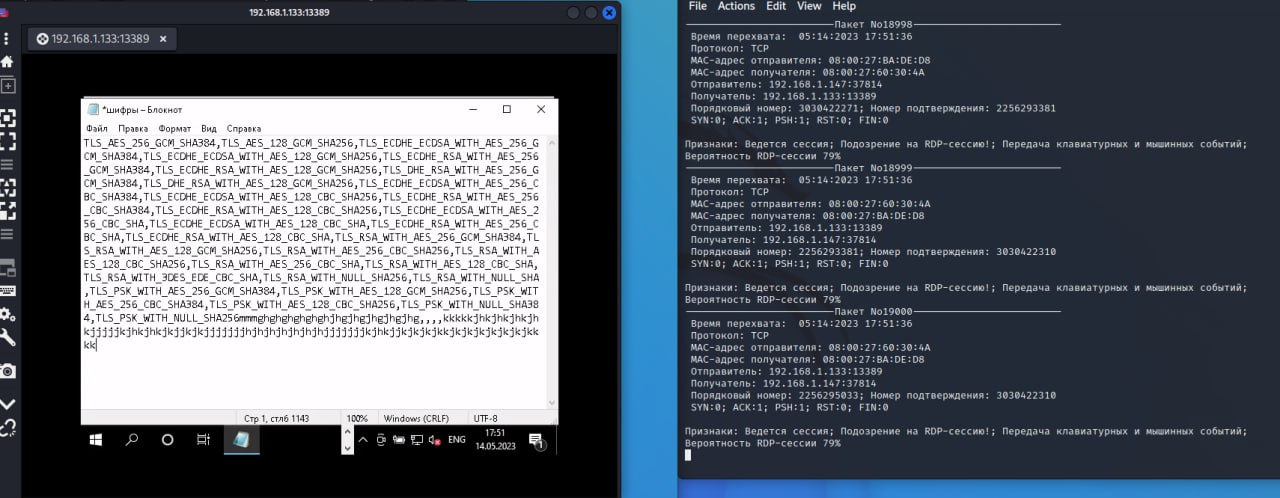
\includegraphics[width=0.8\textwidth]{photo/rdpport4.jpg}
  \caption{Увеличение вероятности RDP-сессии}
  \label{rdpport4}
\end{figure}

Стоит отметить, что если процентное соотношение временных интервалов достигает больше 70\%, то каждый следующий интервал программа
относит к признакам RDP-сессии до самого ее завершения или прерывания.

Далее будет рассмотрено пара примеров работы программы, в которых отсутствует RDP-сессия.

В качестве экперимента была запущена дополнительная ВМ Windows 10 (192.168.1.84), в которой была папка. К ней был предоставлен
общий доступ и в нее же был добавлен файл размером около 6 МБ, как показано
на рисунке \ref{smb-win1}.

\begin{figure}[H]
  \centering
  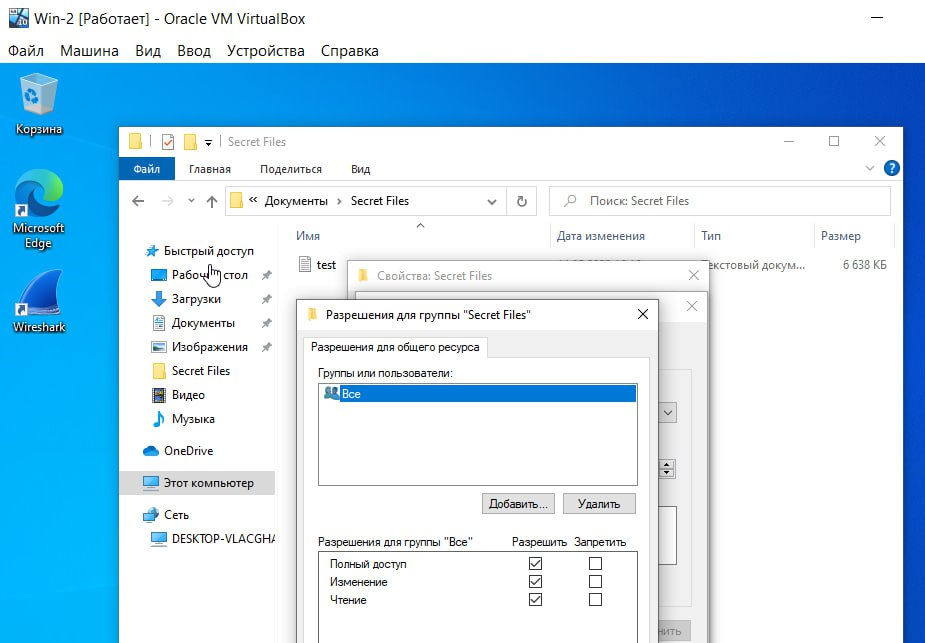
\includegraphics[width=0.8\textwidth]{photo/smb-win1.jpg}
  \caption{Предоставление папке общего доступа}
  \label{smb-win1}
\end{figure}

На следующем рисунке видно, что ВМ Windows 10 (192.168.1.133) имеет доступ к этой папке.

\begin{figure}[H]
  \centering
  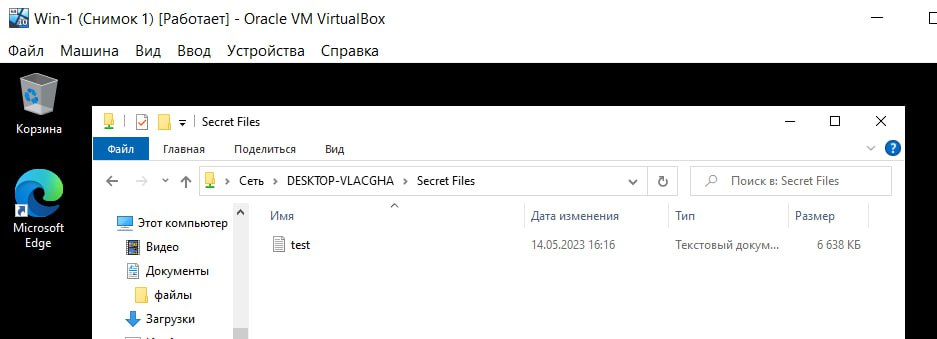
\includegraphics[width=0.8\textwidth]{photo/smb-win2.jpg}
  \caption{Рабочий стол ВМ Windows 10 (192.168.1.133)}
  \label{smb-win2}
\end{figure}

Эксперимент заключается в том, что ВМ Windows 10 (192.168.1.133) должна сохранить к себе файл, находящейся в общей папке.
А в этот момент должна быть запущена программа <<traffic-detection.py>> в режиме перехвата трафика. И необходимо проверить
найдет ли она что-нибудь в данной ситуации. Для начала опыт проводился с выключенным фильтром RDP. Т.е. программа выводила в
консоль абсолютно все пакеты, которые ей удалось перехватить.

В момент перехвата сетевого трафика была установлена сессия, в которой применялся порт 445, как показано на рисунке \ref{smb1}.
Данный порт принадлежит протоколу SMB (Server Message Block). Это протокол сетевого уровня, который используется для обмена 
файлами, печати и других ресурсов между компьютерами в сети. Он является одним из стандартных протоколов Windows и используется 
для обмена данными между компьютерами под управлением Windows.


\begin{figure}[H]
  \centering
  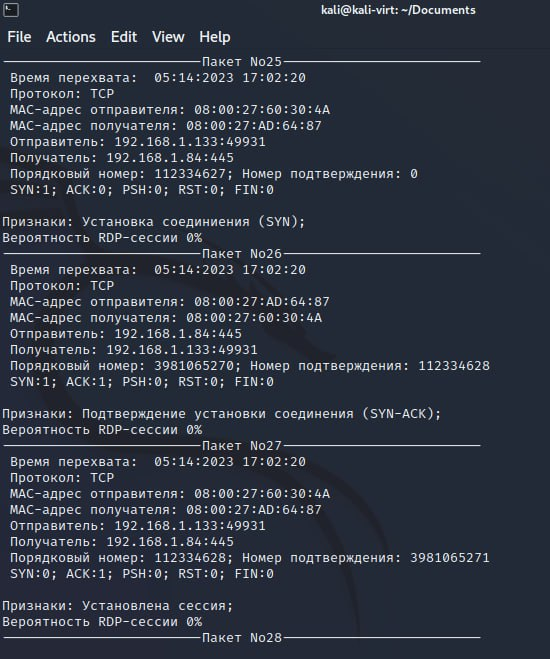
\includegraphics[width=0.8\textwidth]{photo/smb1.jpg}
  \caption{Информация об установке SMB-сессии}
  \label{smb1}
\end{figure}

Из рисунка \ref{smb1} видно, что программа перехватила установку активной SMB-сессии. На следующем рисунке изображен SMB-трафик,
из которого видно, что никаких признаков протокола RDP не наблюдалось.


\begin{figure}[H]
  \centering
  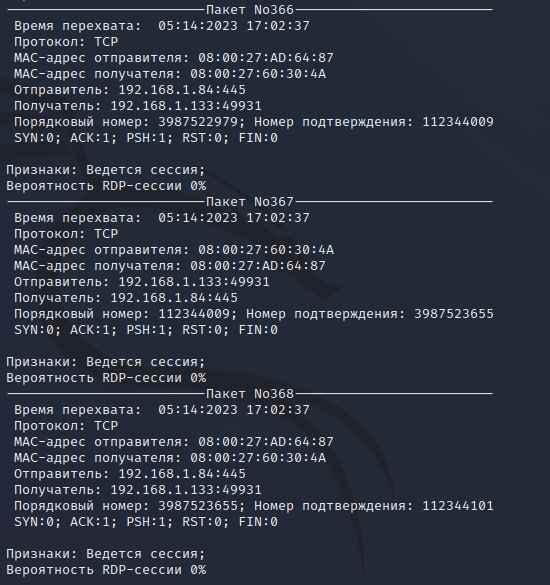
\includegraphics[width=0.8\textwidth]{photo/smb2.jpg}
  \caption{Информация о перехваченных пакетах, принадлежащих SMB-сессии}
  \label{smb2}
\end{figure}

Далее были выполнены аналогичные действия, но перехват трафика осуществлялся уже с включенным фильтром RDP.
На рисунке \ref{smbfilter} показан результат перехвата сетевого трафика.

\begin{figure}[H]
  \centering
  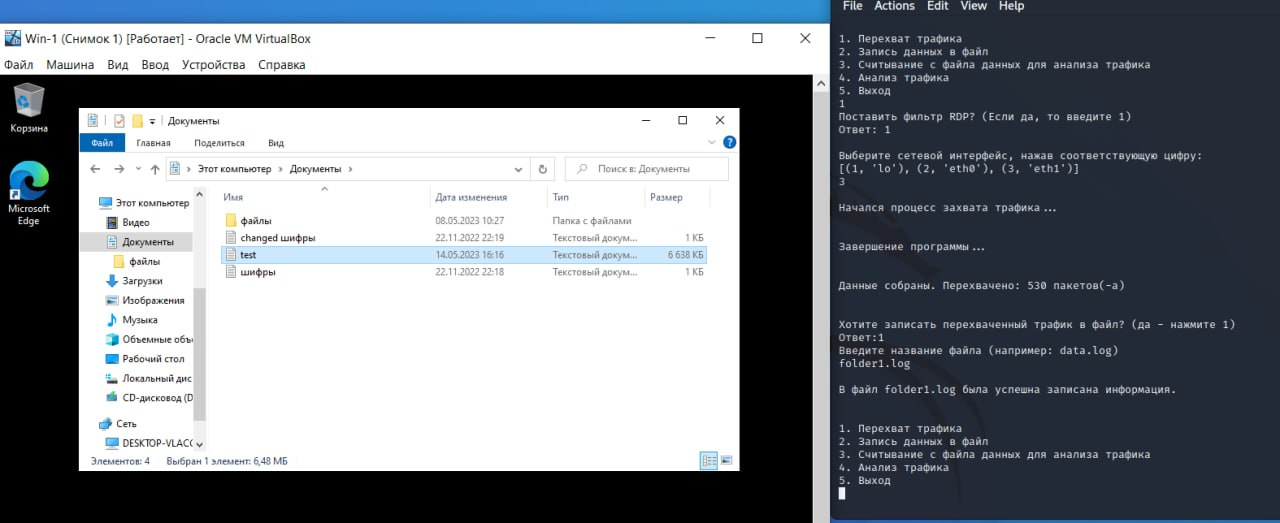
\includegraphics[width=0.9\textwidth]{photo/smb-filter.jpg}
  \caption{Работа программы с установленном фильтром RDP при SMB-сессии}
  \label{smbfilter}
\end{figure}

Согласно рисунку, изображенному на \ref{smbfilter}, программе не удалось обнаружить пакеты, свойственные протоколу RDP, 
так как в данном случае они отсутствовали.   

Следующим шагом будет проведен эксперимент, чтобы выяснить, вызывает ли программа <<traffic-detection.py>> ложные срабатывания 
при обработке HTTP- и HTTPS-трафика. Сначала был запущен перехват сетевого трафика с установленным фильтром RDP. После этого
производилось активное взаимодействие с браузером. На рисунке \ref{http} изображено открытие в интернет-браузере сайта <<Википедия>>, и
пока что никаких ложных срабатываний программы не обнаружено.

\begin{figure}[H]
  \centering
  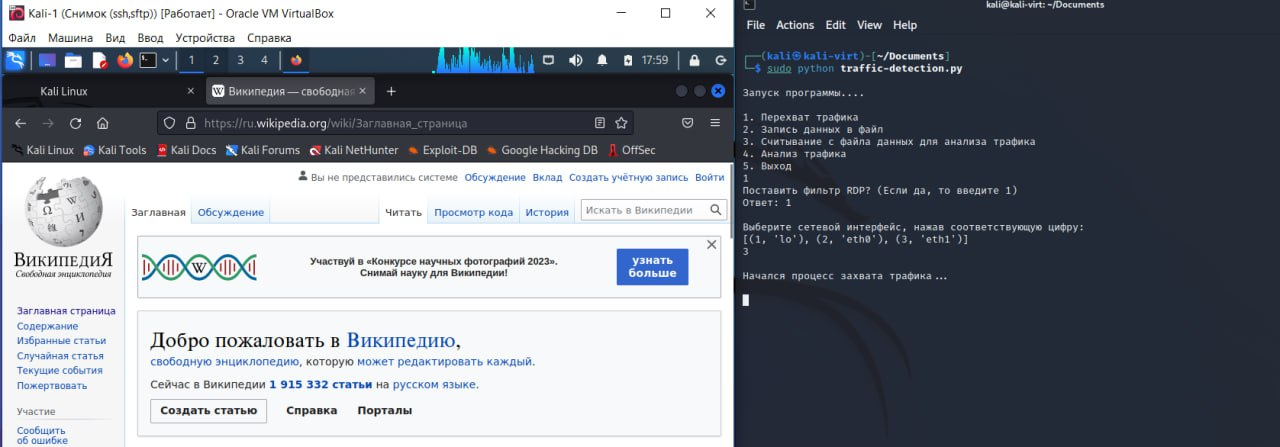
\includegraphics[width=0.9\textwidth]{photo/http.jpg}
  \caption{Перехват трафика при работе с интернет-браузером}
  \label{http}
\end{figure}

В течение нескольких минут в браузере открывались различные вкладки, на которых производились активные движения мышкой И
нажатия клавиш на клавиатуре. Также на некоторых сайтах осуществлялся просмотр видео. 
Из рисунка \ref{http1} видно, что после завершения перехвата сетевого трафика было получено 38347 пакетов, и среди них программа 
не обнаружила признаков активной RDP-сессии. 

\begin{figure}[H]
  \centering
  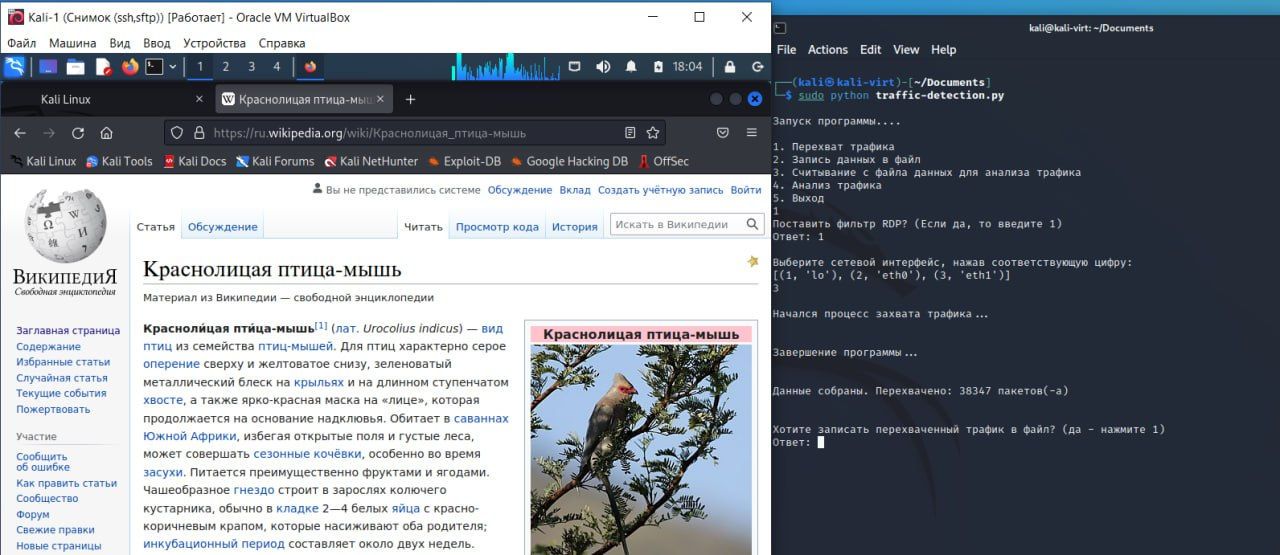
\includegraphics[width=0.8\textwidth]{photo/http2.jpg}
  \caption{Завершение перехвата трафика с установленным фильтром RDP}
  \label{http1}
\end{figure}

Конечно, в данном трафике есть небольшой процент пакетов, которые можно отнести к признакам протокола RDP,
но программа оценивает все пятисекундные интервалы и считает процентное соотношение для каждой установленной активной сессии.


Таким образом, с помощью статистических методов анализа сетевого трафика, реализованных в программе <<traffic-detection.py>>, можно
отличить RDP-трафик от других видов трафика. При всех четырех типах соединений программе удалось верно определить как наличие активных RDP-сессии,
так и их отсутствие. Однако всё равно нельзя однозначно обнаружить RDP-трафик, так как применение статистических методов анализа сетевого трафика
имеет ряд проблем:

\begin{itemize}
  \item Неоднородность трафика: сетевой трафик может содержать множество различных типов трафика, включая RDP-трафик, и использование статистических 
  методов для обнаружения конкретной сессии может оказаться сложным из-за этой неоднородности.
  \item Сложность обработки трафика: RDP-сессии могут содержать множество пакетов, и анализ большого объема трафика может быть сложным и требовать 
  значительных вычислительных ресурсов.
  \item Вариации в сетевых конфигурациях: настройки сетевой конфигурации могут влиять на формат и содержание RDP-трафика, что может затруднить 
  обнаружение RDP-сессий с помощью методов анализа трафика.
\end{itemize}

\conclusion
  
В ходе данной курсовой работы был произведен анализ сетевого трафика для обнаружения активной RDP-сессии с использованием статистических методов. 
Была разработана программная реализация метода, включающая анализ TCP-соединения, обработку данных и построение графиков для анализа поведения 
RDP-трафика. 

Был произведен анализ распределения размера пакетов, вычисление среднего значения и стандартного отклонения размеров пакетов, определение 
верхней и нижней границ диапазона значений размеров пакетов для каждого интервала времени и анализ полученных данных на наличие признаков 
RDP-сессии. Также был проведен анализ распределения временных интервалов между пакетами и частоты флагов PSH.

Были предложены модификации для улучшения обнаружения RDP-сессии, такие как изменение пороговых значений для интервалов и использование 
множественных методов анализа.

Была произведена проверка разработанной программы на определение наличия или отсутствия RDP-сессии, которая показала эффективность 
разработанного метода и программной реализации.

Таким образом, на основе анализа статистических характеристик сетевого трафика была разработана методика обнаружения RDP-сессии, 
которая может быть использована в качестве средства безопасности для защиты информации в компьютерных сетях. 
Рекомендуется дальнейшее исследование и развитие данного метода для его применения в различных условиях и сценариях использования.

  \begin{thebibliography}{15}
    \bibitem{2}
    Удалённый рабочий стол RDP: как включить и как подключиться по RDP [Электронный ресурс] / URL:https://hackware.ru/?p=11835 (дата обращения 31.03.2023), Яз. рус.
    \bibitem{userdp1}
    How to use remote desktop [Электронный ресурс] / URL: https://support.microsoft.com/en-us/windows/how-to-use-remote-desktop-5fe128d5-8fb1-7a23-3b8a-41e636865e8c (дата обращения 27.05.2022), Яз. англ.
    \bibitem{rdp2}
    Документация Remote Utilities <<RDP>> [Электронный ресурс] / URL:  https://www.remoteutilities.com/support/docs/rdp/ (дата обращения 31.03.2023), Яз. англ.
    \bibitem{osi-model}
    Статья <<Модель OSI>> [Электронный ресурс] / URL: http://neerc.ifmo.ru/wiki/index.php?title=OSI_Model (дата обращения 31.03.2023), Яз. рус.
    \bibitem{tcpflags}
    Статья <<TCP flags>> [Электронный ресурс] / URL: https://www.keycdn.com/support/tcp-flags\#:~:text=ACK
    (дата обращения 31.03.2023), Яз. англ.
    \bibitem{socket1}
    Документация по стандартным библиотекам языка Python [Электронный ресурс] / URL: https://docs.python.org/3/library/socket.html (дата обращения 31.03.2023), Яз. англ.
    \bibitem{session} 
    Документация Microsoft <<How Terminal Services Works>> [Электронный ресурс] / URL:  https://learn.microsoft.com/en-us/previous-versions/windows/it-pro/windows-server-2003/cc755399(v=ws.10)?redirectedfrom=MSDN (дата обращения 14.04.2023), Яз. англ.
    \bibitem{rdp1}
    Статья <<Работа с клиентом удаленного рабочего стола Remmina>> [Электронный ресурс] / URL: https://white55.ru/remmina.html
    (дата обращения 15.04.2023), Яз. рус.
    \bibitem{rdpport}
    Документация Microsoft <<Изменение порта прослушивания для удаленного рабочего стола на компьютере>> [Электронный ресурс] / URL: https://learn.microsoft.com/ru-ru/windows-server/remote/remote-desktop-services/clients/change-listening-port
    (дата обращения 28.04.2023), Яз. рус.
    \bibitem{dev0}
    Методическая разработка <<Исследование трафика локальной сети посредством сетевого анализатора <<Wireshark>> >> [Электронный ресурс] / URL: http://ib.psuti.ru/content/metod/методическиеWireshark.pdf
    (дата обращения 04.05.2023), Яз. рус.
    \bibitem{dev1}
    Статья из википедии <<Standard deviation>> [Электронный ресурс] / URL: https://en.wikipedia.org/wiki/Standard\_deviation
    (дата обращения 04.05.2023), Яз. англ.
    \bibitem{dev2}
    Статья <<Стандартное отклонение>> [Электронный ресурс] / URL: https://berg.com.ua/indicators-overlays/stdev/
    (дата обращения 04.05.2023), Яз. рус.

  \end{thebibliography}

  \appendix

    \section{Код traffic-detection.py}
    \inputminted[fontsize=\footnotesize, linenos]{Python}{code/traffic-detection.py}


\end{document}